\documentclass[twocolumn,amsfonts,showpacs,superscriptaddress]{revtex4-1}
%\documentclass[amsfonts,showpacs,superscriptaddress]{revtex4-1}
%\documentclass[10pt,prl,aps,twocolumn,showpacs,superscriptaddress]{revtex4}
\usepackage[dvipdfmx]{graphicx}
\usepackage{amssymb,amsmath,amsthm,booktabs,mathtools}
%\usepackage{floatflt}
\usepackage{bbm}
\usepackage{bm}% bold math
\usepackage{color}
\usepackage[colorlinks,bookmarks=false,citecolor=blue,linkcolor=red,urlcolor=blue]{hyperref}
\usepackage{tikz}
\usepackage{pgfplots}
\usepackage{enumitem}

\def\ben#1{{\color{blue} #1}}

%\def\tit#1{{\em #1},}
\def\etal#1{#1}

\def\tit#1{}
%\def\etal#1{ {\em et al.}}
\newcommand{\half}{{\textstyle\frac{1}{2}}}
\newcommand{\nhalf}{{\frac{1}{2}}}
\newcommand{\nthalf}{{\frac{3}{2}}}
\newcommand{\nfhalf}{{\frac{5}{2}}}
\newcommand{\thalf}{{\textstyle\frac{3}{2}}}
\newcommand{\quart}{{\textstyle\frac{1}{4}}}
\newcommand{\iquart}{{\textstyle\frac{\ii}{4}}}
\usepackage{color}
\def\red#1{\textcolor{red}{#1}}
\DeclareMathOperator{\End}{End}
\DeclareMathOperator{\lsp}{lsp}
\newcommand{\Mod}[1]{\ (\mathrm{mod}\ #1)}







\newcommand{\comJ}[1]{{\color{orange}#1}}

% Définir une couleur grise personnalisée
\definecolor{mygray}{gray}{0.3}
\definecolor{myblue}{rgb}{0, 0, 0.5}
\definecolor{myred}{rgb}{0.5, 0, 0}

% Nouvelle commande pour les traductions
%\newcommand{\trad}[1]{\textcolor{mygray}{#1}}
\newcommand{\trad}[1]{\textcolor{myblue}{#1}}

\newcommand{\resumefr}[1]{\textcolor{myred}{#1}}




\usepackage{amsmath}	% required for `\align' (yatex added)
\begin{document}

\title{Quantum Generalized Hydrodynamics\\
\trad{Hydrodynamique Généralisée Quantique} }



\author{Paola Ruggiero}
\affiliation
{SISSA and INFN, Via Bonomea 265, 34136 Trieste, Italy}
\author{Pasquale Calabrese}
\affiliation
{SISSA and INFN, Via Bonomea 265, 34136 Trieste, Italy}
\affiliation
{International Centre for Theoretical Physics (ICTP), Strada Costiera 11, 34151 Trieste, Italy}
\author{Benjamin Doyon}
\affiliation
{Department of Mathematics, King’s College London, Strand WC2R 2LS, UK}
\author{J\'er\^ome Dubail}
\affiliation
{Laboratoire de Physique et Chimie Th\'eoriques, CNRS, UMR 7019, Universit\'e de Lorraine, 54506 Vandoeuvre-les-Nancy, France
}



\begin{abstract}
Physical systems made of many interacting quantum particles can often be described by Euler hydrodynamic equations in the limit of long wavelengths and low frequencies. Recently such a classical hydrodynamic framework, now dubbed {\it Generalized Hydrodynamics} (GHD), was found for quantum integrable models in one spatial dimension. Despite its great predictive power, GHD, like any Euler hydrodynamic equation, misses important quantum effects, such as quantum fluctuations leading to non-zero equal-time correlations between fluid cells at different positions. Focusing on the one-dimensional gas of bosons with delta repulsion, and on states of zero entropy, for which quantum fluctuations are larger, we reconstruct such quantum effects by quantizing GHD. The resulting theory of {\it quantum GHD} can be viewed as a multi-component Luttinger liquid theory, with a small set of effective parameters that are fixed by the Thermodynamic Bethe Ansatz. It describes quantum fluctuations of truly nonequilibrium systems where conventional Luttinger liquid theory fails.
\trad{
Les systèmes physiques composés de nombreuses particules quantiques en interaction peuvent souvent être décrits par des équations hydrodynamiques d'Euler dans la limite des longues longueurs d'onde et des basses fréquences. Récemment, un tel cadre hydrodynamique classique, désormais baptisé {\it Hydrodynamique Généralisée} (GHD), a été trouvé pour les modèles quantiques intégrables dans une dimension spatiale. Malgré son grand pouvoir prédictif, la GHD, comme toute équation hydrodynamique d'Euler, manque des effets quantiques importants, tels que les fluctuations quantiques menant à des corrélations de temps égal non nulles entre les cellules de fluide à différentes positions. En se concentrant sur le gaz unidimensionnel de bosons avec répulsion delta, et sur des états de zéro entropie, pour lesquels les fluctuations quantiques sont plus importantes, nous reconstruisons ces effets quantiques en quantifiant la GHD. La théorie résultante de la {\it GHD quantique} peut être vue comme une théorie des liquides de Luttinger multi-composants, avec un petit ensemble de paramètres effectifs fixés par l'Ansatz Thermodynamique de Bethe. Elle décrit les fluctuations quantiques de systèmes véritablement hors d'équilibre où la théorie conventionnelle des liquides de Luttinger échoue.}	
\end{abstract}



\maketitle


The behavior of fluids at very low temperatures is usually peculiar as the quantum nature of their constituents dominates over thermal fluctuations. To describe collective quantum effects, it is customary to start from classical hydrodynamic equations, and to quantize them. This path was taken by Landau in 1941~\cite{landau1941theory} in his development of the theory of superfluid helium \cite{khalatnikov2018introduction,putterman1974superfluid}. Since then, similar approaches have been developed for various other quantum liquids~\cite{nozieres2018theory,leggett2006quantum}, including for instance Bose-Einstein condensates where quantum fluctuations are captured by the Bogoliubov theory~\cite{bogolyubov1947theory,pitaevskii2016bose,mora2003extension}, quantum Hall liquids~\cite{wiegmann2013hydrodynamics,wiegmann2014anomalous,wiegmann2019quantization}, 
or one-dimensional (1d) quantum fluids described by Luttinger liquid theory~\cite{haldane1981luttinger,giamarchi2003quantum,cazalilla2004bosonizing}.
\trad{Le comportement des fluides à très basses températures est généralement particulier car la nature quantique de leurs constituants domine sur les fluctuations thermiques. Pour décrire les effets quantiques collectifs, il est courant de partir des équations hydrodynamiques classiques, puis de les quantifier. Cette approche a été suivie par Landau en 1941 dans le cadre du développement de la théorie de l'hélium superfluide. Depuis lors, des approches similaires ont été développées pour divers autres liquides quantiques, y compris par exemple les condensats de Bose-Einstein, où les fluctuations quantiques sont capturées par la théorie de Bogolioubov, les liquides quantiques de Hall, ou les fluides quantiques unidimensionnels décrits par la théorie du liquide de Luttinger.}



The purpose of this Letter is to apply a similar program to the classical hydrodynamics of one-dimensional quantum integrable models introduced in 2016~\cite{bertini2016transport,castro2016emergent}, now dubbed {\it Generalized Hydrodynamics} (GHD). At equilibrium, the Luttinger
liquid theory ---which is the quantized hydrodynamic theory
of 1d fluids~\cite{abanov2006hydrodynamics} with few conserved quantities such
as charge, magnetization, energy, momentum--- is enough to capture
quantum fluctuations of 1d gapless integrable models~\cite{haldane1981luttinger,giamarchi2003quantum,cazalilla2004bosonizing}. However,
when dealing with true out-of-equilibrium situations, like the quantum Newton's cradle setup~\cite{kinoshita2006quantum} ---whose hydrodynamics description must keep track of all higher conservations laws~\cite{rigol2007relaxation}, and is provided by GHD~\cite{caux2019hydrodynamics}---, quantum fluctuations must be given by a more general quantum hydrodynamics theory, obtainable by quantizing GHD.
Here our goal is to identify that theory.
\trad{Le but de cette Lettre est d'appliquer un programme similaire à l'hydrodynamique classique des modèles quantiques intégrables unidimensionnels introduits en 2016~\cite{bertini2016transport,castro2016emergent}, désormais appelés {\it Hydrodynamique Généralisée} (GHD). À l'équilibre, la théorie du liquide de Luttinger, qui est la théorie hydrodynamique quantifiée des fluides unidimensionnels~\cite{abanov2006hydrodynamics} avec quelques grandeurs conservées telles que la charge, la magnétisation, l'énergie et le moment, suffit pour capturer les fluctuations quantiques des modèles intégrables unidimensionnels sans gap~\cite{haldane1981luttinger,giamarchi2003quantum,cazalilla2004bosonizing}. Cependant, lorsqu'il s'agit de situations réellement hors d'équilibre, comme le montage expérimental de la bille de Newton quantique~\cite{kinoshita2006quantum}, dont la description hydrodynamique doit prendre en compte toutes les lois de conservation supérieures~\cite{rigol2007relaxation}, cela est assuré par la GHD~\cite{caux2019hydrodynamics}. Les fluctuations quantiques doivent alors être décrites par une théorie d'hydrodynamique quantique plus générale, obtenue en quantifiant la GHD. Notre objectif ici est d'identifier cette théorie.}



\begin{figure}[!h]%ht
	%\begin{tikzpicture}[scale=0.5]
		%\draw (-1,0) node{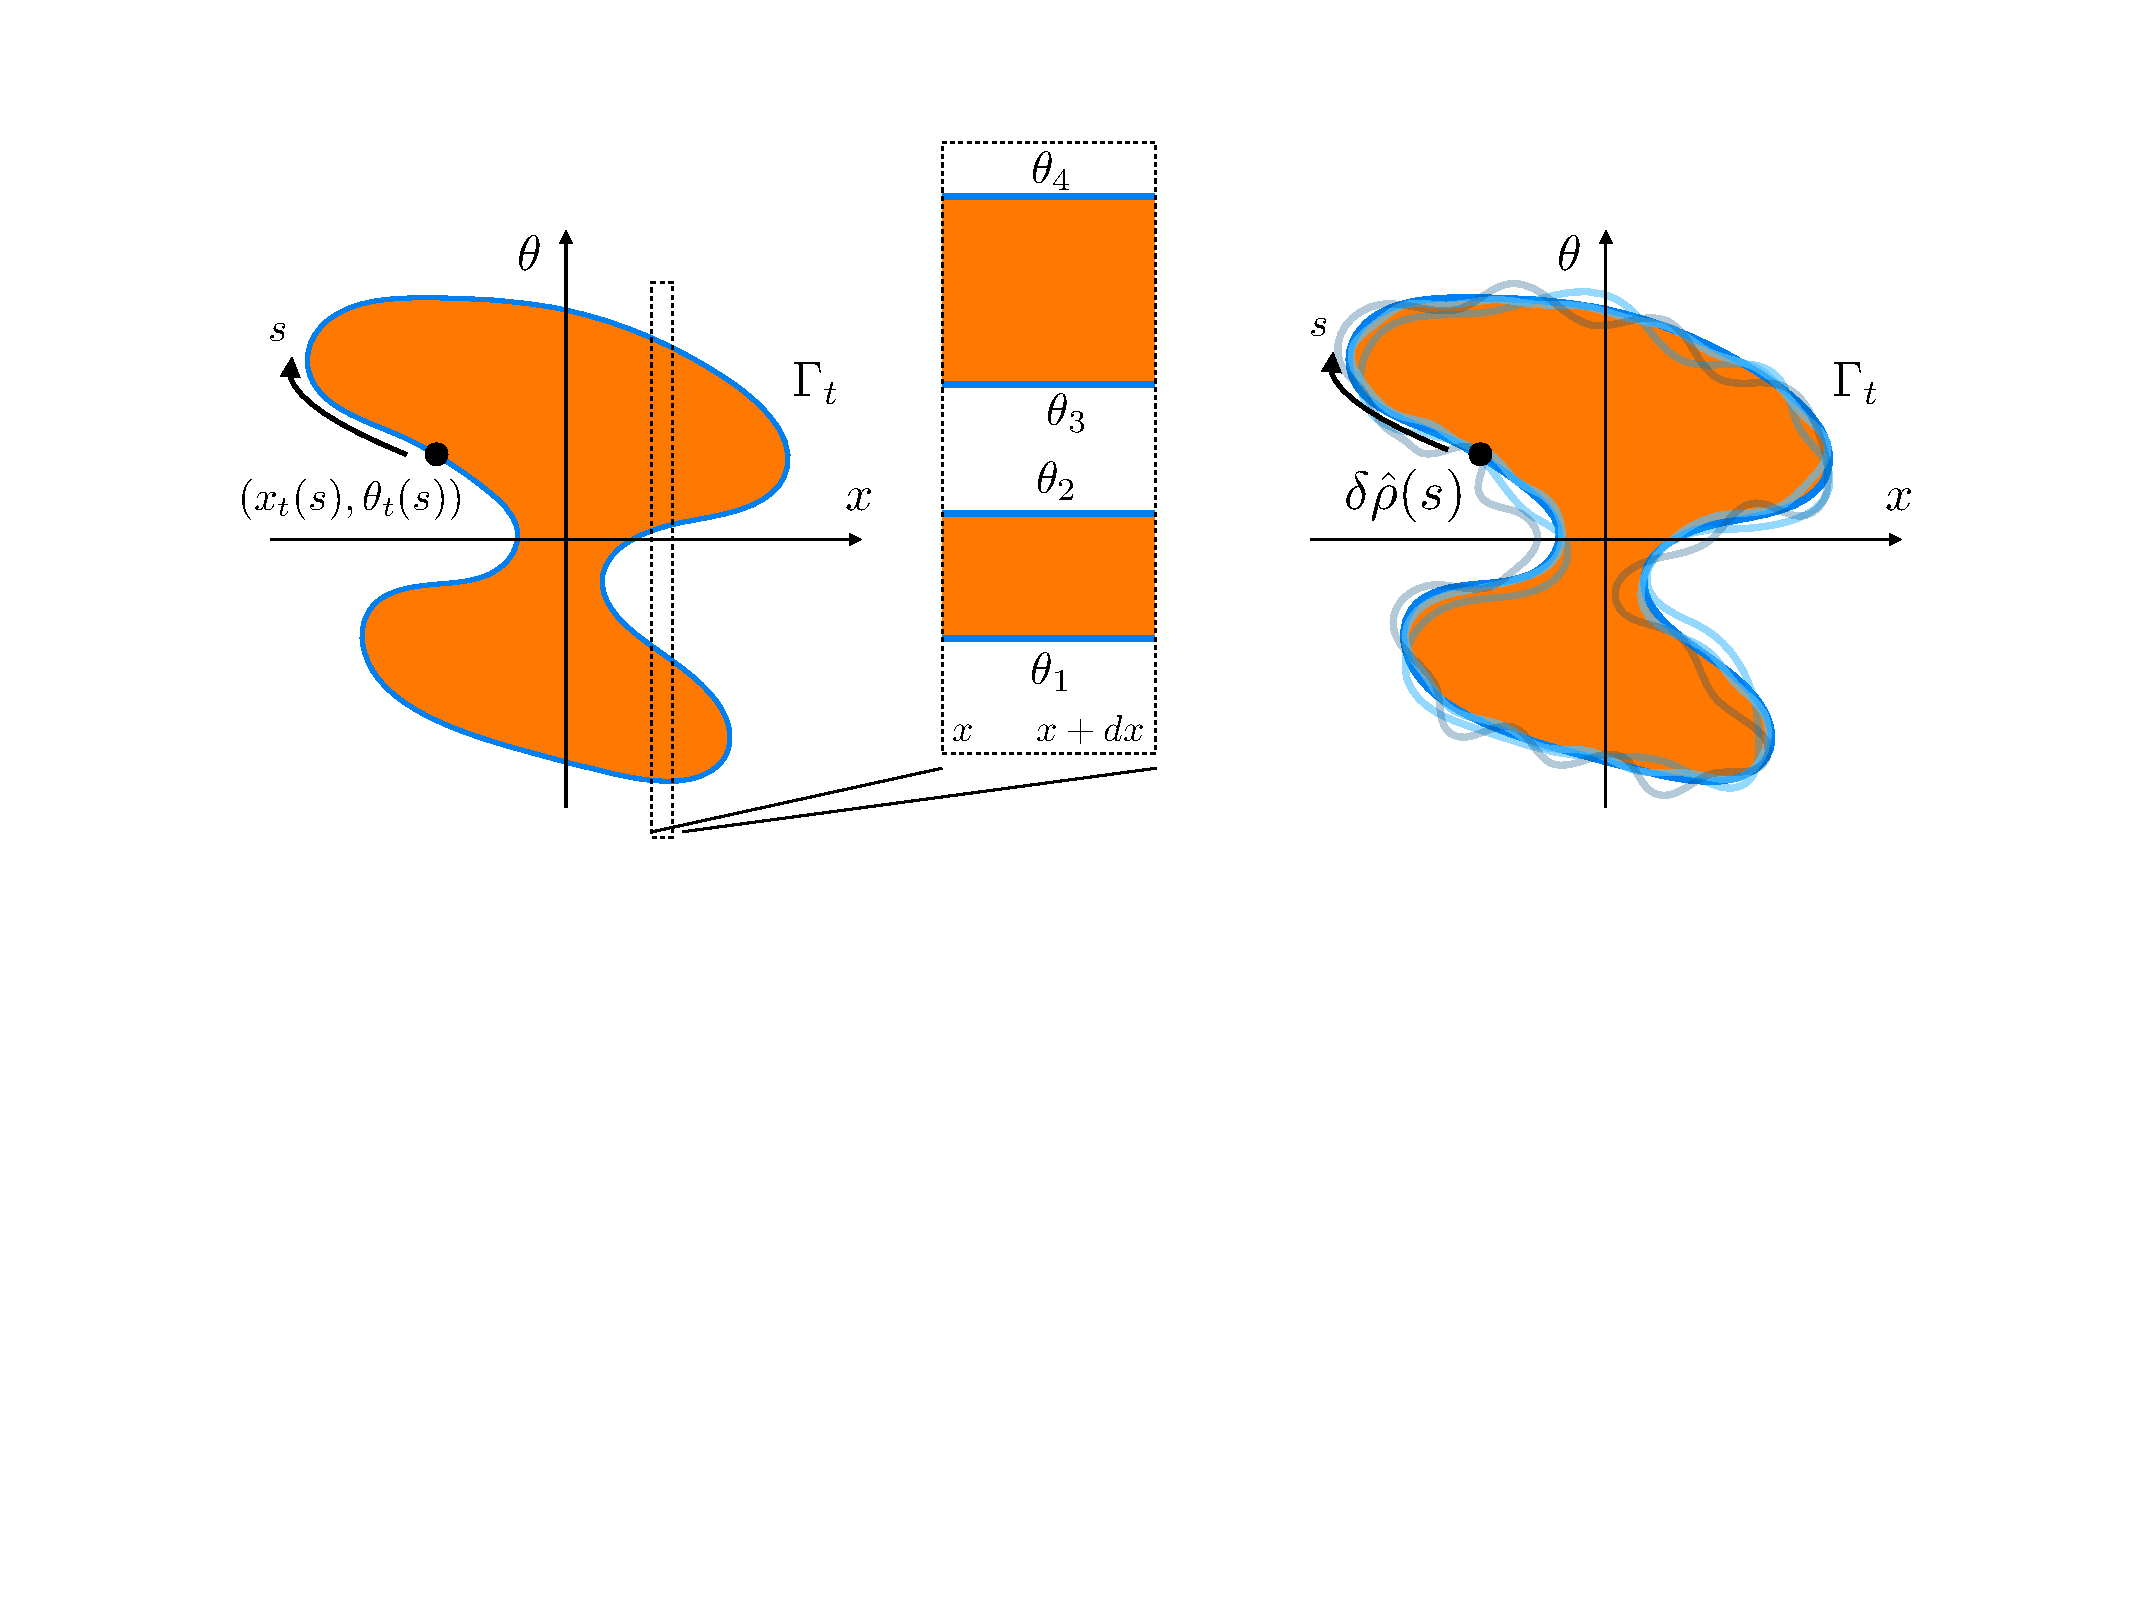
\includegraphics[width=0.48\textwidth]{fig1.pdf}};
		%\draw (-8,-3) node{$a)$};
		%\draw (3,-3) node{$b)$};
	%\end{tikzpicture}
	\tikz \draw (0,0) node {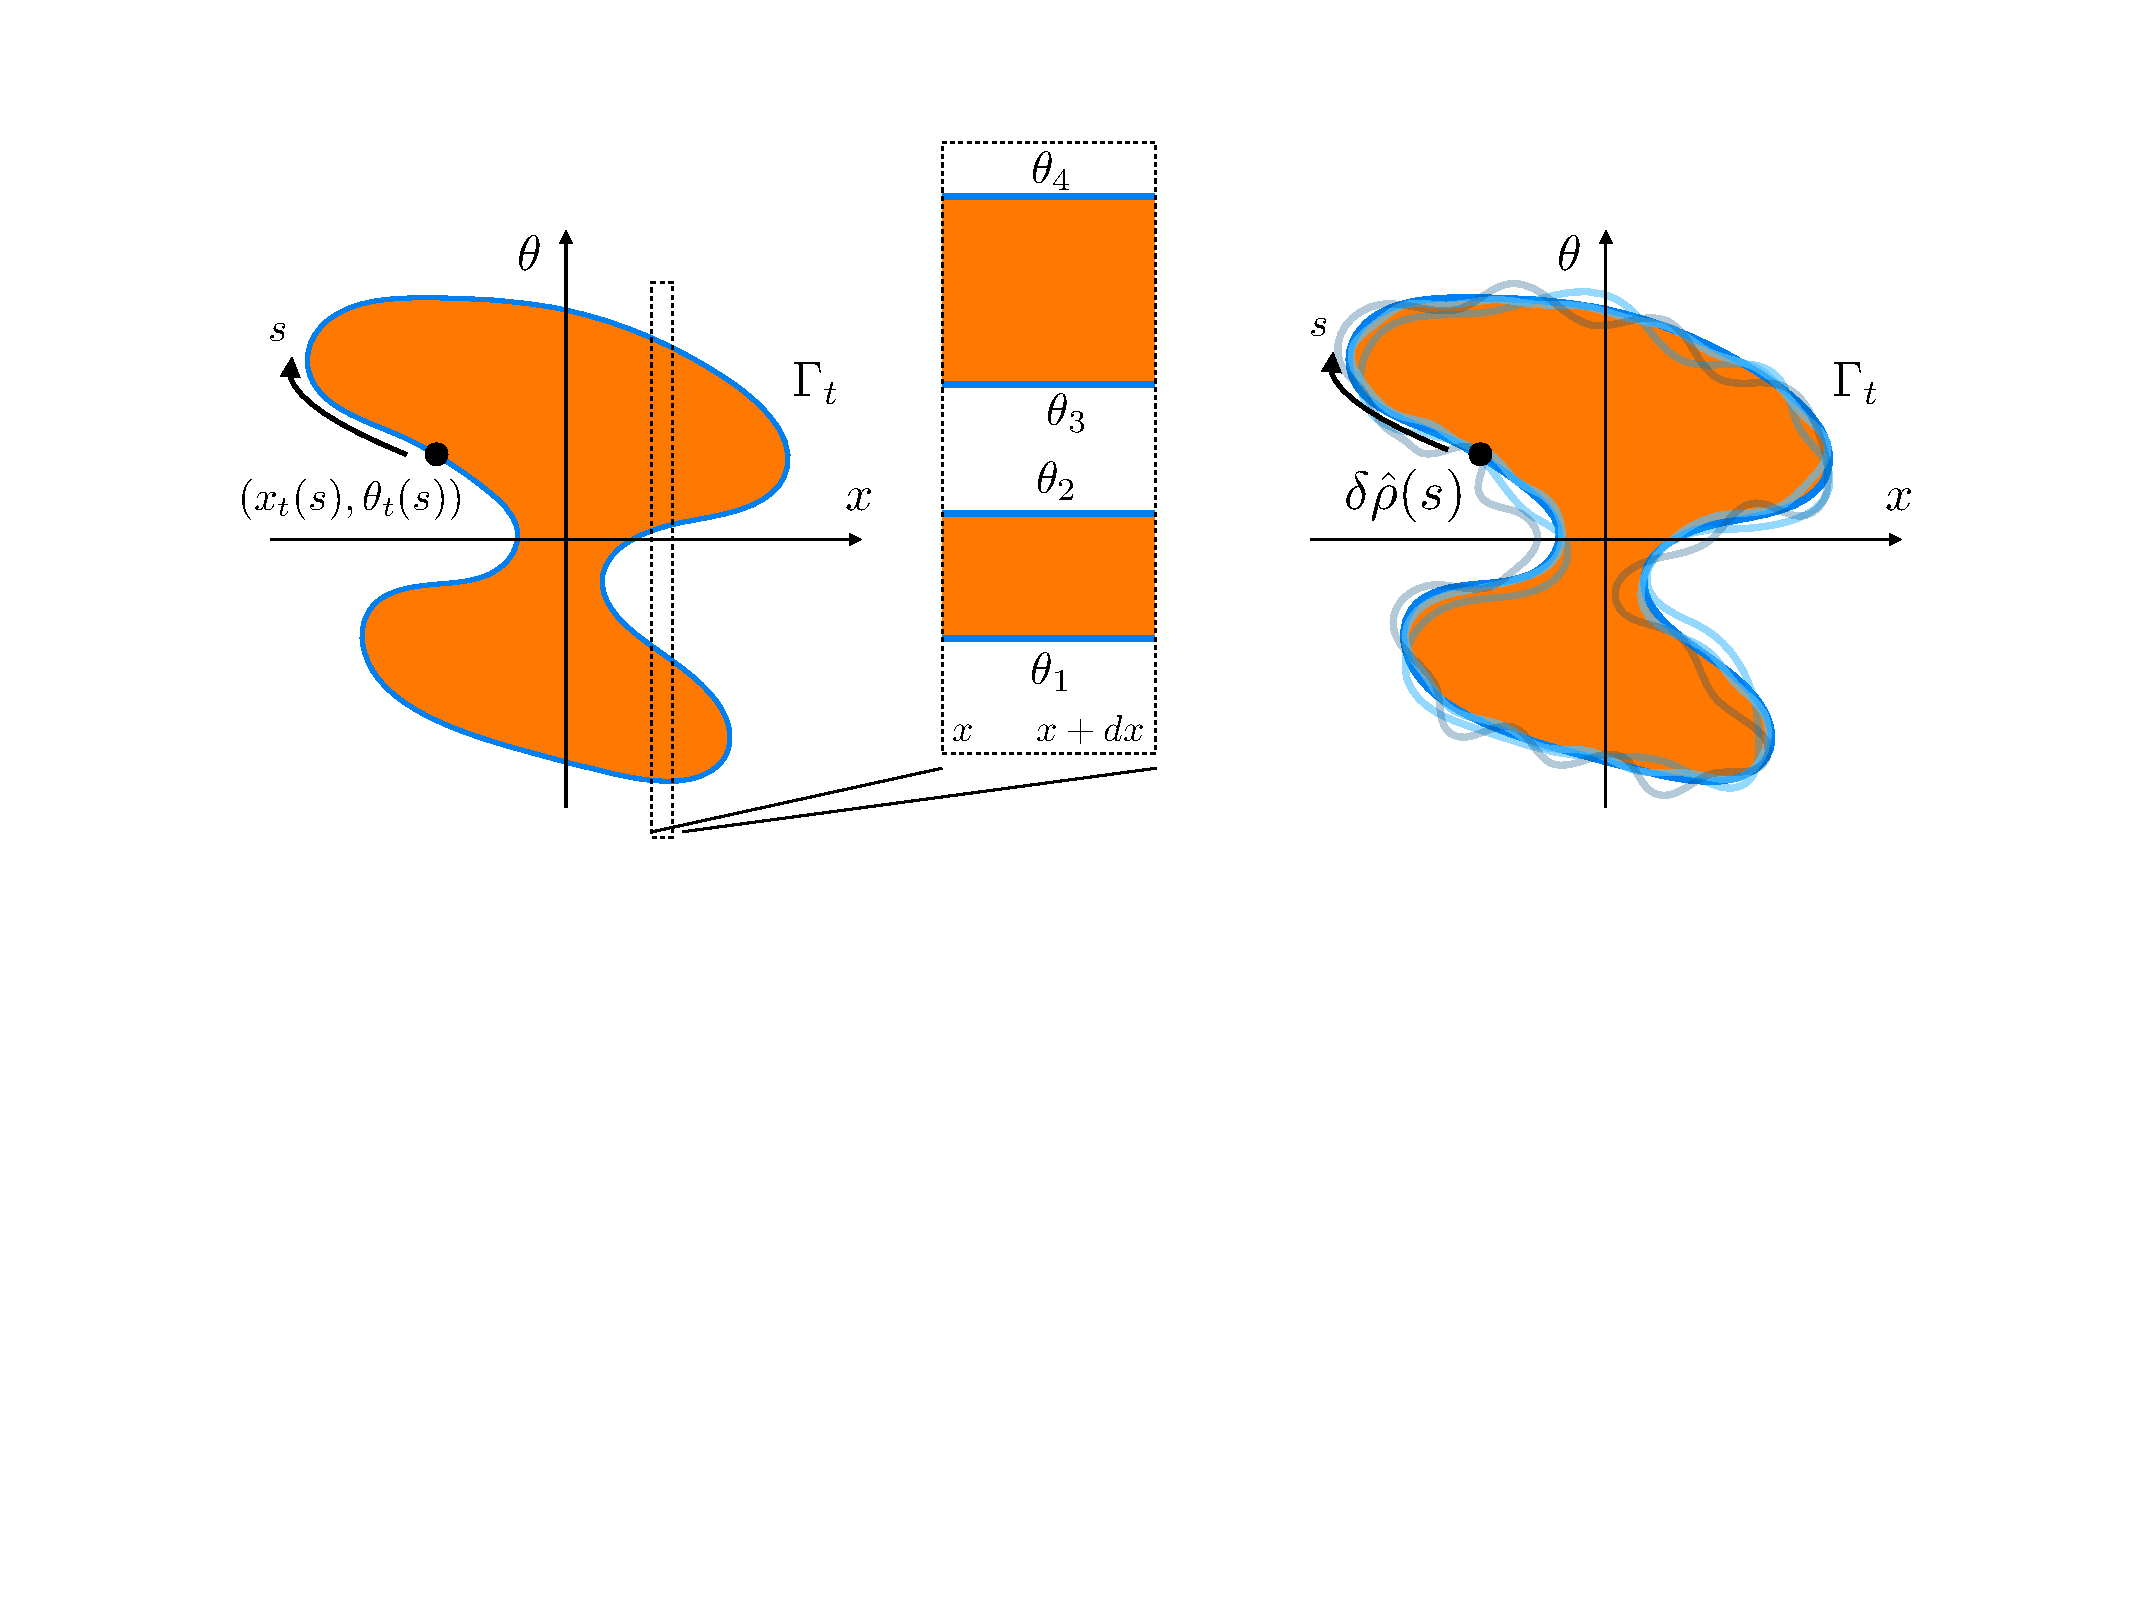
\includegraphics[width=0.48\textwidth]{fig1.pdf}} (0,0) node {$a)$} (5,0) node {$b)$};

	\vspace{-0.6cm}
	\caption{(a) Zero-entropy GHD describes the motion of the Fermi contour $\Gamma_t$, parametrized as in Eq. (\ref{eq:params}), which separates the regions in phase space where the Fermi factor $n(x,\theta)$ is one (orange) or zero (white) at a given time $t$. In any small interval $[x,x+ d x]$ the fluid is in a state called {\it split Fermi sea} \cite{fokkema2014split,eliens2016general,vlijm2016correlations,eliens2017quantum} labeled by Fermi rapidities $\theta_1 < \theta_2 < \dots < \theta_{2q}$; the number of fluid components $q$ is a piecewise constant function of $x$ and $t$. (b) In this Letter the contour $\Gamma_t$ is allowed to have quantum fluctuations around the classical solution to the zero-entropy GHD equations (\ref{eq:GHD}a-b). The quantum fluctuations are captured by a chiral boson with density $\delta \hat{\rho} (s)$ living along the contour.
	\trad{(a) La GHD à entropie nulle décrit le mouvement du contour de Fermi \(\Gamma_t\), paramétré comme dans l'équation (\ref{eq:params}), qui sépare les régions de l'espace des phases où le facteur de Fermi \(n(x,\theta)\) est un (orange) ou zéro (blanc) à un instant donné \(t\). Dans tout petit intervalle \([x,x+ dx]\), le fluide est dans un état appelé {\it mer de Fermi scindée} \cite{fokkema2014split,eliens2016general,vlijm2016correlations,eliens2017quantum} caractérisé par des rapidités de Fermi \(\theta_1 < \theta_2 < \dots < \theta_{2q}\); le nombre de composants du fluide \(q\) est une fonction constante par morceaux de \(x\) et \(t\). (b) Dans cette Lettre, le contour \(\Gamma_t\) est autorisé à avoir des fluctuations quantiques autour de la solution classique des équations de GHD à entropie nulle (\ref{eq:GHD}a-b). Les fluctuations quantiques sont capturées par un boson chirale avec une densité \(\delta \hat{\rho} (s)\) vivant le long du contour.}
	}
	\label{fig:Fermi}
\end{figure}

Our starting point is GHD, which, on the technical side, relies on the formalism of the Thermodynamic Bethe Ansatz~\cite{yang1969thermodynamics,takahashi2005thermodynamics}. Thermodynamically large integrable systems are described by densities of different species of quasiparticles. For simplicity,
in this Letter we formulate our results in a specific model: the 1d Bose gas with delta repulsion~\cite{lieb1963exact,berezin1964schrodinger,korepin1997quantum}. This model is singled out because of its experimental relevance ---it is routinely used for describing contemporary cold atom experiments in 1d~\cite{olshanii1998atomic,van2008yang,vogler2013thermodynamics,schemmer2019generalized,wilson2019observation}--- and because of its simple thermodynamics involving a {\it single} species of quasiparticles. Our approach can be straightforwardly generalized to other integrable systems with a GHD description~\cite{piroli2017transport,ilievski2017microscopic,ilievski2017ballistic,doyon2017large,doyon2017drude,bulchandani2018bethe,collura2018analytic,doyon2018soliton,cao2018incomplete,doyon2018exact,bastianello2018generalized,de2018hydrodynamic,10.21468/SciPostPhys.6.4.049,gopalakrishnan2018hydrodynamics,mazza2018energy,vu2018equations,borsi2019current,doyon2019generalised,bulchandani2019kinetic,spohn2019generalized,bastianello2019generalized,panfil2019linearized,alba2019towards,agrawal2019generalized,cubero2019generalized,bertini2019GHD,mestyan2019GHD,bertini2018GHD,bertini2019GHDb,mestyan2019GHDb}, including for instance the XXZ chain; we defer mathematical formulas for the general multi-species case to the Supplemental Material (SM)~\cite{SM}.
\trad{Notre point de départ est la GHD, qui, sur le plan technique, repose sur le formalisme de l'Ansatz Thermodynamique de Bethe~\cite{yang1969thermodynamics,takahashi2005thermodynamics}. Les grands systèmes intégrables thermodynamiques sont décrits par des densités de différentes espèces de quasi-particules. Pour simplifier, dans cette Lettre, nous formulons nos résultats dans un modèle spécifique : le gaz de Bose unidimensionnel avec répulsion delta~\cite{lieb1963exact,berezin1964schrodinger,korepin1997quantum}. Ce modèle est mis en avant en raison de sa pertinence expérimentale — il est couramment utilisé pour décrire les expériences contemporaines sur les atomes froids en 1d~\cite{olshanii1998atomic,van2008yang,vogler2013thermodynamics,schemmer2019generalized,wilson2019observation} — et en raison de sa thermodynamique simple impliquant une {\it seule} espèce de quasi-particules. Notre approche peut être facilement généralisée à d'autres systèmes intégrables avec une description GHD~\cite{piroli2017transport,ilievski2017microscopic,ilievski2017ballistic,doyon2017large,doyon2017drude,bulchandani2018bethe,collura2018analytic,doyon2018soliton,cao2018incomplete,doyon2018exact,bastianello2018generalized,de2018hydrodynamic,10.21468/SciPostPhys.6.4.049,gopalakrishnan2018hydrodynamics,mazza2018energy,vu2018equations,borsi2019current,doyon2019generalised,bulchandani2019kinetic,spohn2019generalized,bastianello2019generalized,panfil2019linearized,alba2019towards,agrawal2019generalized,cubero2019generalized,bertini2019GHD,mestyan2019GHD,bertini2018GHD,bertini2019GHDb,mestyan2019GHDb}, y compris par exemple la chaîne XXZ ; nous remettons les formules mathématiques pour le cas général multi-espèces dans le Matériel Supplémentaire (SM)~\cite{SM}.}




At the microscopic level, the 1d Bose gas with delta repulsion is defined by the Hamiltonian for $N$ bosons $H = \sum_{i=1}^N [-\frac{\hbar^2}{2} \partial_{x_i}^2 + V(x_i)] + \hbar \bar{g} \sum_{i<j} \delta(x_i-x_j) $, where $g = \hbar \bar{g} >0$ is the repulsion strength between the bosons and $V(x)$ is an external trapping potential. 
We set the mass of the bosons to $1$. 
\trad{Au niveau microscopique, le gaz de Bose unidimensionnel avec répulsion delta est défini par l'hamiltonien pour \( N \) bosons :
\[ H = \sum_{i=1}^N \left[ -\frac{\hbar^2}{2} \partial_{x_i}^2 + V(x_i) \right] + \hbar \bar{g} \sum_{i<j} \delta(x_i-x_j), \]
où \( \bar{g} = \frac{g}{\hbar} > 0 \) est la force de répulsion entre les bosons, \( V(x) \) est un potentiel de piégeage externe, et nous avons fixé la masse des bosons à \( 1 \).
}

GHD is formulated at the Euler scale, where space-time scales of observations and length scales of external potentials are simultaneously sent to infinity; at the Euler scale diffusion is absent (but subleading diffusive corrections to GHD are also known  \cite{de2018hydrodynamic,10.21468/SciPostPhys.6.4.049,gopalakrishnan2018hydrodynamics}). In the 1d Bose gas the Euler scale is equivalently expressed as the  classical limit~\cite{brun2017one,brun2018inhomogeneous,ruggiero2019conformal}
\begin{equation}
	\label{eq:limit}
	 \hbar \rightarrow 0 , \quad \; {\rm keeping} \quad \hbar N, \; V(x), \; \bar{g} \; \; {\rm fixed }.
\end{equation}
For the gas starting at {\it zero temperature}, its evolution under GHD takes a particularly simple form~\cite{doyon2017large}. Indeed, an initial zero-temperature state has zero entropy and entropy is conserved by Euler equations such as GHD. [This is generally true for Euler hydrodynamic equations away from shocks, and it is known that GHD does not admit shocks~\cite{el2005kinetic,doyon2017large,bulchandani2017classical}.] Thus the Bose fluid remains locally in a macrostate with zero entropy at all times. In the Bose gas with delta repulsion, the presence of higher conservation laws allows for a large space of macrostates with zero entropy: the {\it split Fermi seas}~\cite{fokkema2014split,eliens2016general,vlijm2016correlations,eliens2017quantum}. They can be labeled by a set of {\it Fermi rapidities} $\{\theta_a\}_{1\leq a\leq 2q}$ such that the {\it Fermi factor} $n(\theta)$ ---the number of Bethe quasiparticles with rapidity in $[\theta, \theta + d \theta]$ divided by the number of available states in that interval (see e.g. Chap. 1 in Ref.~\cite{korepin1997quantum}  for an introduction to that formalism)--- is
\begin{equation}
	n(\theta) \, = \, \left\{ \begin{array}{rcl} 
		1 & {\rm if} & \theta \in [\theta_1 ,\theta_2] \cup \dots \cup [\theta_{2q-1},\theta_{2q}] \\
		0 & & {\rm otherwise} .
		\end{array}
	 \right.
\end{equation}
The local macrostate is then assumed to be a function of position $x$ and of time $t$. The global state of the system at time $t$ is best represented by the {\it Fermi contour} $\Gamma_t$ (see Fig. \ref{fig:Fermi}), which is defined such that the Fermi factor $n(x,\theta)$ is $1$ for all points $(x,\theta)$ inside the contour, and $0$ outside. For simplicity we restrict to situations where $\Gamma_t$ is a simple closed curve, parametrized by a function $s \mapsto (x_t(s), \theta_t(s))$,
\begin{equation}
	\label{eq:params}
	\Gamma_t = \{ (x_t(s), \theta_t(s)) , s \in  \mathbb{R}/ 2\pi \mathbb{Z} \}  .
\end{equation}
According to GHD, the time evolution of the contour $\Gamma_t$ is given by the classical equation~\cite{doyon2017large}
\begin{subequations}
	\label{eq:GHD}
\begin{equation}
	\frac{d}{dt} \left( \begin{array}{c}
		x_t(s) \\
		\theta_t(s)
	\end{array} \right) \, = \,  \left( \begin{array}{c}
		v^{\rm eff} (x_t(s),\theta_t(s))  \\
		a^{\rm eff}(x_t(s),\theta_t(s))
 	\end{array} \right) ,
\end{equation}
which expresses the fact that quasiparticles inside the contour move at an effective velocity $v^{\rm eff}(x,\theta)$ and are accelerated at an effective acceleration $a^{\rm eff}(x,\theta)$, both of which depend in general on the local Hamiltonian and macrostate, hence on the Fermi points at $x$. Eq. (\ref{eq:GHD}a) is complemented by a closed formula for the effective velocity~\cite{bonnes2014light,bertini2016transport,castro2016emergent,vu2019equations} and acceleration~\cite{doyon2017note}
\begin{equation}
	v^{\rm eff}  \, = \, (\partial_\theta E)^{\rm dr} / 1^{\rm dr}   ,\quad
	a^{\rm eff}  \, = \, -(\partial_xE)^{\rm dr} / 1^{\rm dr} ,
\end{equation}
\end{subequations}
where $E(x,\theta)$ is the bare energy of a quasiparticle with respect to the local Hamiltonian, $1(\theta) = 1$, and the {\it dressing} of a function $f(\theta)$ in the local macrostate is defined by the integral equation $f^{\rm dr} (\theta) \, = \, f(\theta) +  \int \frac{d\theta'}{2\pi} \frac{d \phi (\theta-\theta')}{d \theta} n(\theta') f^{\rm dr} (\theta')$. Here $\phi(\theta-\theta') = 2 \, {\rm arctan} \left( (\theta-\theta')/\bar{g} \right)$ is the two-body scattering phase for the delta Bose gas~\cite{lieb1963exact,berezin1964schrodinger,korepin1997quantum}. In the present case, $E(x,\theta) = \theta^2/2 + V(x)$, and the effective acceleration simplifies to give Newton's second law~\cite{doyon2017note}
\begin{equation}
	\label{eq:newton}
	a^{\rm eff}= -\partial_x V(x).
\end{equation}
Notice that $\hbar$ is completely absent from the Eqs. (\ref{eq:GHD}a,b), which is consistent with our claim that zero-entropy GHD corresponds to the classical limit (\ref{eq:limit}) in the microscopic model.
\trad{La GHD est formulée à l'échelle d'Euler, où les échelles spatio-temporelles des observations et les échelles de longueur des potentiels externes sont simultanément envoyées à l'infini ; à l'échelle d'Euler, la diffusion est absente (mais des corrections diffusives subalternes à la GHD sont également connues \cite{de2018hydrodynamic,10.21468/SciPostPhys.6.4.049,gopalakrishnan2018hydrodynamics}). Dans le gaz de Bose 1d, l'échelle d'Euler est équivalente à la limite classique~\cite{brun2017one,brun2018inhomogeneous,ruggiero2019conformal}
\begin{equation*}
	%\label{eq:limit}
	 \hbar \rightarrow 0 , \quad \; \text{en maintenant} \quad \hbar N, \; V(x), \; \bar{g} \; \; \text{fixés}.
\end{equation*}
Pour le gaz démarrant à {\it température nulle}, son évolution sous la GHD prend une forme particulièrement simple~\cite{doyon2017large}. En effet, un état initial à température nulle a une entropie nulle et l'entropie est conservée par les équations d'Euler telles que la GHD. [Cela est généralement vrai pour les équations hydrodynamiques d'Euler loin des chocs, et il est connu que la GHD n'admet pas de chocs~\cite{el2005kinetic,doyon2017large,bulchandani2017classical}.] Ainsi, le fluide de Bose reste localement dans un macro-état à entropie nulle à tout moment. Dans le gaz de Bose avec répulsion delta, la présence de lois de conservation supérieures permet un grand espace de macro-états à entropie nulle : les {\it mers de Fermi scindées}~\cite{fokkema2014split,eliens2016general,vlijm2016correlations,eliens2017quantum}. Elles peuvent être étiquetées par un ensemble de {\it rapidités de Fermi} $\{\theta_a\}_{1\leq a\leq 2q}$ tel que le {\it facteur de Fermi} $n(\theta)$ — le nombre de quasi-particules de Bethe avec une rapidité dans $[\theta, \theta + d \theta]$ divisé par le nombre d'états disponibles dans cet intervalle (voir par exemple le Chap. 1 de Ref.~\cite{korepin1997quantum} pour une introduction à ce formalisme) — est
\begin{equation*}
	n(\theta) \, = \, \left\{ 
	    \begin{array}{rcl} 
		    1 & \text{si} & \theta \in [\theta_1 ,\theta_2] \cup \dots \cup [\theta_{2q-1},\theta_{2q}] \\
		    0 & & \text{autrement} .
		\end{array}
	 \right.
\end{equation*}
Le macro-état local est alors supposé être une fonction de la position $x$ et du temps $t$. L'état global du système au temps $t$ est mieux représenté par le {\it contour de Fermi} $\Gamma_t$ (voir Fig. \ref{fig:Fermi}), qui est défini de sorte que le facteur de Fermi $n(x,\theta)$ soit $1$ pour tous les points $(x,\theta)$ à l'intérieur du contour, et $0$ à l'extérieur. Pour simplifier, nous nous limitons aux situations où $\Gamma_t$ est une courbe fermée simple, paramétrée par une fonction $s \mapsto (x_t(s), \theta_t(s))$,
\begin{equation*}
	%\label{eq:params}
	\Gamma_t = \{ (x_t(s), \theta_t(s)) , s \in  \mathbb{R}/ 2\pi \mathbb{Z} \}  .
\end{equation*}
Selon la GHD, l'évolution temporelle du contour $\Gamma_t$ est donnée par l'équation classique~\cite{doyon2017large}
\begin{subequations}
	%\label{eq:GHD}
	\begin{equation*}
		\frac{d}{dt} \left( 
		    \begin{array}{c}
			    x_t(s) \\
			    \theta_t(s)
		    \end{array} 
		\right) \, = \,  
		\left( 
		    \begin{array}{c}
			    v^{\rm eff} (x_t(s),\theta_t(s))  \\
			    a^{\rm eff}(x_t(s),\theta_t(s))
		    \end{array} 
		\right) ,
	\end{equation*}
	qui exprime le fait que les quasi-particules à l'intérieur du contour se déplacent à une vitesse effective $v^{\rm eff}(x,\theta)$ et sont accélérées à une accélération effective $a^{\rm eff}(x,\theta)$, toutes deux dépendant en général de l'hamiltonien local et du macro-état, donc des points de Fermi à $x$. L'équation (\ref{eq:GHD}a) est complétée par une formule fermée pour la vitesse effective~\cite{bonnes2014light,bertini2016transport,castro2016emergent,vu2019equations} et l'accélération~\cite{doyon2017note}
	\begin{equation*}
		v^{\rm eff}  \, = \, (\partial_\theta E)^{\rm dr} / 1^{\rm dr} , \quad
		a^{\rm eff}  \, = \, -(\partial_xE)^{\rm dr} / 1^{\rm dr} ,
	\end{equation*}
\end{subequations}
où $E(x,\theta)$ est l'énergie nue d'une quasi-particule par rapport à l'hamiltonien local, $1(\theta) = 1$, et le {\it habillage} d'une fonction $f(\theta)$ dans le macro-état local est défini par l'équation intégrale $f^{\rm dr} (\theta) \, = \, f(\theta) +  \int \frac{d\theta'}{2\pi} \frac{d \phi (\theta-\theta')}{d \theta} n(\theta') f^{\rm dr} (\theta')$. Ici, $\phi(\theta-\theta') = 2 \, \text{arctan} \left( (\theta-\theta')/\bar{g} \right)$ est la phase de diffusion à deux corps pour le gaz de Bose delta~\cite{lieb1963exact,berezin1964schrodinger,korepin1997quantum}. Dans le cas présent, $E(x,\theta) = \theta^2/2 + V(x)$, et l'accélération effective se simplifie pour donner la deuxième loi de Newton~\cite{doyon2017note}
\begin{equation*}
	%\label{eq:newton}
	a^{\rm eff}= -\partial_x V(x).
\end{equation*}
Remarquez que $\hbar$ est complètement absent des équations (\ref{eq:GHD}a,b), ce qui est cohérent avec notre affirmation selon laquelle la GHD à entropie nulle correspond à la limite classique (\ref{eq:limit}) dans le modèle microscopique.
}

\vspace{0.1cm} \noindent {\bf\em Goal of this Letter.}\; Because it is a classical hydrodynamic description, GHD misses certain quantum effects, such as quantum entanglement or correlations between the different parts of the fluid at a given time. Such effects appear as subleading orders in an expansion at small $\hbar$ in the limit (\ref{eq:limit}). Here we initiate the development of a theory of {\it quantum fluctuations around GHD}. Analogously to Bogoliubov theory~\cite{bogolyubov1947theory,pitaevskii2016bose,mora2003extension}, our strategy is to start from linear sound waves propagating on top of a background configuration $(x_t(s), \theta_t(s))$ which solves the GHD equation (Fig.~\ref{fig:Fermi}), and then find a way to quantize those. We find that the resulting theory takes the form of a {\it time-dependent, spatially inhomogeneous, multi-component Luttinger liquid}, which generalizes the effective theory of (homogeneous, time-independent) split Fermi seas developed recently by Eli\"ens and Caux~\cite{eliens2016general}, see also Refs.~\cite{fokkema2014split,vlijm2016correlations,eliens2017quantum}. It also generalizes the theory of inhomogeneous Luttinger liquids (see e.g. Refs.~\cite{gangardt2003stability,abanov2006hydrodynamics,dubail2017conformal,brun2017one,brun2018inhomogeneous,ruggiero2019conformal,cazalilla2004bosonizing}) to truly out-of-equilibrium situations, like the situation depicted in  Fig.~\ref{movie} (see the discussion below).
\trad{\vspace{0.1cm} \noindent {\bf\em Objectif de cette lettre.}\; Étant donné qu'il s'agit d'une description hydrodynamique classique, la GHD omet certains effets quantiques, tels que l'entrelacement quantique ou les corrélations entre les différentes parties du fluide à un moment donné. De tels effets apparaissent comme des ordres subalternes dans une expansion en petites valeurs de \( \hbar \) dans la limite (\ref{eq:limit}). Ici, nous entamons le développement d'une théorie des {\it fluctuations quantiques autour de la GHD}. De manière analogue à la théorie de Bogolioubov~\cite{bogolyubov1947theory,pitaevskii2016bose,mora2003extension}, notre stratégie est de partir des ondes sonores linéaires se propageant sur une configuration de fond $(x_t(s), \theta_t(s))$ qui résout l'équation de la GHD (voir Fig.~\ref{fig:Fermi}), puis de trouver un moyen de les quantifier. Nous découvrons que la théorie résultante prend la forme d'un {\it liquide de Luttinger multi-composants, spatialement inhomogène et dépendant du temps}, ce qui généralise la théorie effective des mers de Fermi scindées (homogènes, indépendantes du temps) développée récemment par Eli\"ens et Caux~\cite{eliens2016general}, voir aussi Refs.~\cite{fokkema2014split,vlijm2016correlations,eliens2017quantum}. Elle généralise également la théorie des liquides de Luttinger inhomogènes (voir par exemple Refs.~\cite{gangardt2003stability,abanov2006hydrodynamics,dubail2017conformal,brun2017one,brun2018inhomogeneous,ruggiero2019conformal,cazalilla2004bosonizing}) à des situations véritablement hors d'équilibre, comme la situation illustrée dans la Fig.~\ref{movie} (voir la discussion ci-dessous).}


%To illustrate the physical effects that can be attacked with this {\it quantum fluctuating GHD} (QGHD) ---as opposed to GHD--- we consider a quench of the confining potential $V(x)$, from double-well to harmonic, a situation similar to the famous quantum Newton's cradle~\cite{kinoshita2006quantum}. This protocol can be realized experimentally (see e.g. Refs.~\cite{joseph2011observation,schemmer2019generalized}) and produces local macrostates that are split Fermi seas. Comparing the equal-time density-density correlation predicted by QGHD and  find that the predictions of QGHD are in good agreement with the numerics (see Fig.~\ref{movie}). %More results obtainable from QGHD, as well as more extensive numerical checks, will be presented in an extended version of this work~\cite{longversion}. 



\vspace{0.1cm} \noindent {\bf\em Sound waves in zero-entropy GHD.}\; Linearly propagating waves are consequences of the conservation laws of hydrodynamics. By fluctuation-dissipation, they are subject to correlations due to microscopic fluctuations. Thus, our first task is to find conserved fluid modes and their linear-response evolution. Let us parametrise locally the contour $\Gamma_t$ by the Fermi points $\theta_a(x,t)$ ($1 \leq a \leq 2q$). Fluctuations can be expressed as deformations of the contour $\theta_a(x,t)\rightarrow \theta_a(x,t)+\delta \theta_a(x,t)$. Plugging this into Eqs. (\ref{eq:GHD}a,b), one would arrive at an evolution equation for $\delta \theta_a (x,t)$, describing the propagation of sound waves on top of the background solution $(x_t (s) , \theta_t(s) )$. These, however, do not take the form of conservation equations.

Instead, we consider the momentum and energy of an excitation%above a Bethe background
~\cite{korepin1997quantum}, $p(\theta) = \theta + \int \frac{d\theta'}{2\pi} \phi(\theta-\theta') n(\theta')1^{\rm dr}(\theta')$ and $\epsilon(\theta) = E(x,\theta) + \int \frac{d\theta'}{2\pi} \phi(\theta-\theta')n(\theta')1^{\rm dr}(\theta')v^{\rm eff}(\theta')$, respectively. The dispersion relation of such an excitation is the effective velocity, $\partial_\theta \epsilon/ \partial_\theta p = v^{\rm eff}$. In the theory of GHD~\cite{bertini2016transport,castro2016emergent}, any conserved charge of the form $q = \int \frac{d \theta'}{2\pi} f(\theta') n(\theta')1^{\rm dr} (\theta')$, which counts $f(\theta')$ for every quasiparticle $\theta'$, satisfies a continuity equation with the current $j =\int \frac{d \theta'}{2\pi} f(\theta') n(\theta') 1^{\rm dr} (\theta') v^{\rm eff}(\theta')$. In an external potential, the continuity equation includes the effective acceleration (\ref{eq:newton}), see Ref.~\cite{doyon2017note}: $\partial_t q + \partial_x j =  \int \frac{d \theta'}{2\pi} f'(\theta') n(\theta') 1^{\rm dr} (\theta') a^{\rm eff}(\theta')$. We observe that the second terms in the expressions of $p(\theta), \epsilon(\theta)$ are precisely of the form $q, j$ (with $f(\theta') = \phi(\theta-\theta')$ \footnote{This is the ``scattering charge'', counting the total phase accumulated by the $\theta$-quasiparticle.}) therefore the conservation equation with force term holds,
\begin{equation}\label{eq:k}
	\partial_t p + \partial_x \epsilon + a^{\rm eff} 1^{\rm dr} = 0.
\end{equation}
%By the general theory of GHD \cite{bertini2016transport,castro2016emergent}, we observe that the second terms in these expressions {\color{red} are averages of a conserved density and its current.  By inspection, we see that the associated total charge, the ``scattering charge", counts $\phi(\theta-\theta')$ for every quasiparticle of rapidity $\theta'$ in the state: it is the total phase accumulated by the $\theta$-quasiparticle. This indeed shifts the physical momentum $p(\theta)$ as per the Bethe ansatz, and the observation is that its current shifts the physical energy}. Thus, a conservation equation, with force term, holds, 
%\begin{equation}\label{eq:k}
%	\partial_t p + \partial_x \epsilon + a^{\rm eff} 1^{\rm dr}=0.
%\end{equation}
Excitations in a zero-entropy state occur at the Fermi points. Combining the dispersion relation, \eqref{eq:k} and \eqref{eq:GHD}, one finds an {\em exact conservation law} for their momentum $p_a = p(\theta_a)$  and energy $\epsilon_a = \epsilon(\theta_a)$ (see Supplemental Material (SM) for detailed derivation~\cite{SM}):
\begin{equation}\label{eq:ka}
	\partial_t p_a + \partial_x \epsilon_a = 0.
\end{equation}
Then the small fluctuations obey, at first order,
\begin{equation}\label{eq:deltaka}
	\partial_t \delta p_a + \sum_b\partial_x[\mathsf A_a^{~b} \delta p_b] = 0,
\end{equation}
where $ \mathsf A_a^{~b} = \partial \epsilon_a/\partial p_b$ is the {\it flux Jacobian}. This is the propagation equation we were looking for: it is an equation for linear sound waves which takes the form of a conservation equation.
\trad{\vspace{0.1cm} \noindent {\bf\em Ondes sonores dans la GHD à entropie nulle.}\; Les ondes se propageant linéairement sont des conséquences des lois de conservation en hydrodynamique. Par fluctuation-dissipation, elles sont soumises à des corrélations dues aux fluctuations microscopiques. Ainsi, notre première tâche est de trouver les modes de fluide conservés et leur évolution en réponse linéaire. Paramétrons localement le contour $\Gamma_t$ par les points de Fermi $\theta_a(x,t)$ ($1 \leq a \leq 2q$). Les fluctuations peuvent être exprimées comme des déformations du contour $\theta_a(x,t)\rightarrow \theta_a(x,t)+\delta \theta_a(x,t)$. En substituant cela dans les équations (\ref{eq:GHD}a,b), on obtient une équation d'évolution pour $\delta \theta_a(x,t)$, décrivant la propagation des ondes sonores sur la solution de fond $(x_t(s), \theta_t(s))$. Cependant, ces équations ne prennent pas la forme d'équations de conservation.
Nous considérons plutôt le moment et l'énergie d'une excitation au-dessus d'un fond de Bethe~\cite{korepin1997quantum}, $p(\theta) = \theta + \int \frac{d\theta'}{2\pi} \phi(\theta-\theta') n(\theta')1^{\rm dr}(\theta')$ et $\epsilon(\theta) = E(x,\theta) + \int \frac{d\theta'}{2\pi} \phi(\theta-\theta')n(\theta')1^{\rm dr}(\theta')v^{\rm eff}(\theta')$, respectivement. La relation de dispersion de cette excitation est la vitesse effective, $\partial_\theta \epsilon / \partial_\theta p = v^{\rm eff}$. Dans la théorie de la GHD~\cite{bertini2016transport,castro2016emergent}, toute charge conservée de la forme $q = \int \frac{d \theta'}{2\pi} f(\theta') n(\theta')1^{\rm dr} (\theta')$, qui compte $f(\theta')$ pour chaque quasiparticule $\theta'$, satisfait une équation de continuité avec le courant $j = \int \frac{d \theta'}{2\pi} f(\theta') n(\theta') 1^{\rm dr} (\theta') v^{\rm eff}(\theta')$. Dans un potentiel externe, l'équation de continuité inclut l'accélération effective (\ref{eq:newton}), voir Ref.~\cite{doyon2017note} : $\partial_t q + \partial_x j = \int \frac{d \theta'}{2\pi} f'(\theta') n(\theta') 1^{\rm dr} (\theta') a^{\rm eff}(\theta')$. Nous observons que les deuxièmes termes dans les expressions de $p(\theta)$, $\epsilon(\theta)$ sont précisément de la forme $q$, $j$ (avec $f(\theta') = \phi(\theta-\theta')$ \footnote{Il s'agit de la ``charge de diffusion'', comptant la phase totale accumulée par la quasiparticule $\theta$.}) ; par conséquent, l'équation de conservation avec terme de force est valide,
\begin{equation*}%\label{eq:k}
	\partial_t p + \partial_x \epsilon + a^{\rm eff} 1^{\rm dr} = 0.
\end{equation*}
Les excitations dans un état à entropie nulle se produisent aux points de Fermi. En combinant la relation de dispersion, \eqref{eq:k} et \eqref{eq:GHD}, on trouve une {\em loi de conservation exacte} pour leur moment $p_a = p(\theta_a)$ et leur énergie $\epsilon_a = \epsilon(\theta_a)$ (voir le Matériel Supplémentaire (SM) pour une dérivation détaillée~\cite{SM}) :
\begin{equation*}%\label{eq:ka}
	\partial_t p_a + \partial_x \epsilon_a = 0.
\end{equation*}
Ensuite, les petites fluctuations obéissent, au premier ordre,
\begin{equation*}%\label{eq:deltaka}
	\partial_t \delta p_a + \sum_b \partial_x[\mathsf A_a^{~b} \delta p_b] = 0,
\end{equation*}
où $ \mathsf A_a^{~b} = \partial \epsilon_a / \partial p_b$ est le {\it jacobien de flux}. C'est l'équation de propagation que nous recherchions : c'est une équation pour les ondes sonores linéaires qui prend la forme d'une équation de conservation.}


\begin{figure*}[t]
\centering
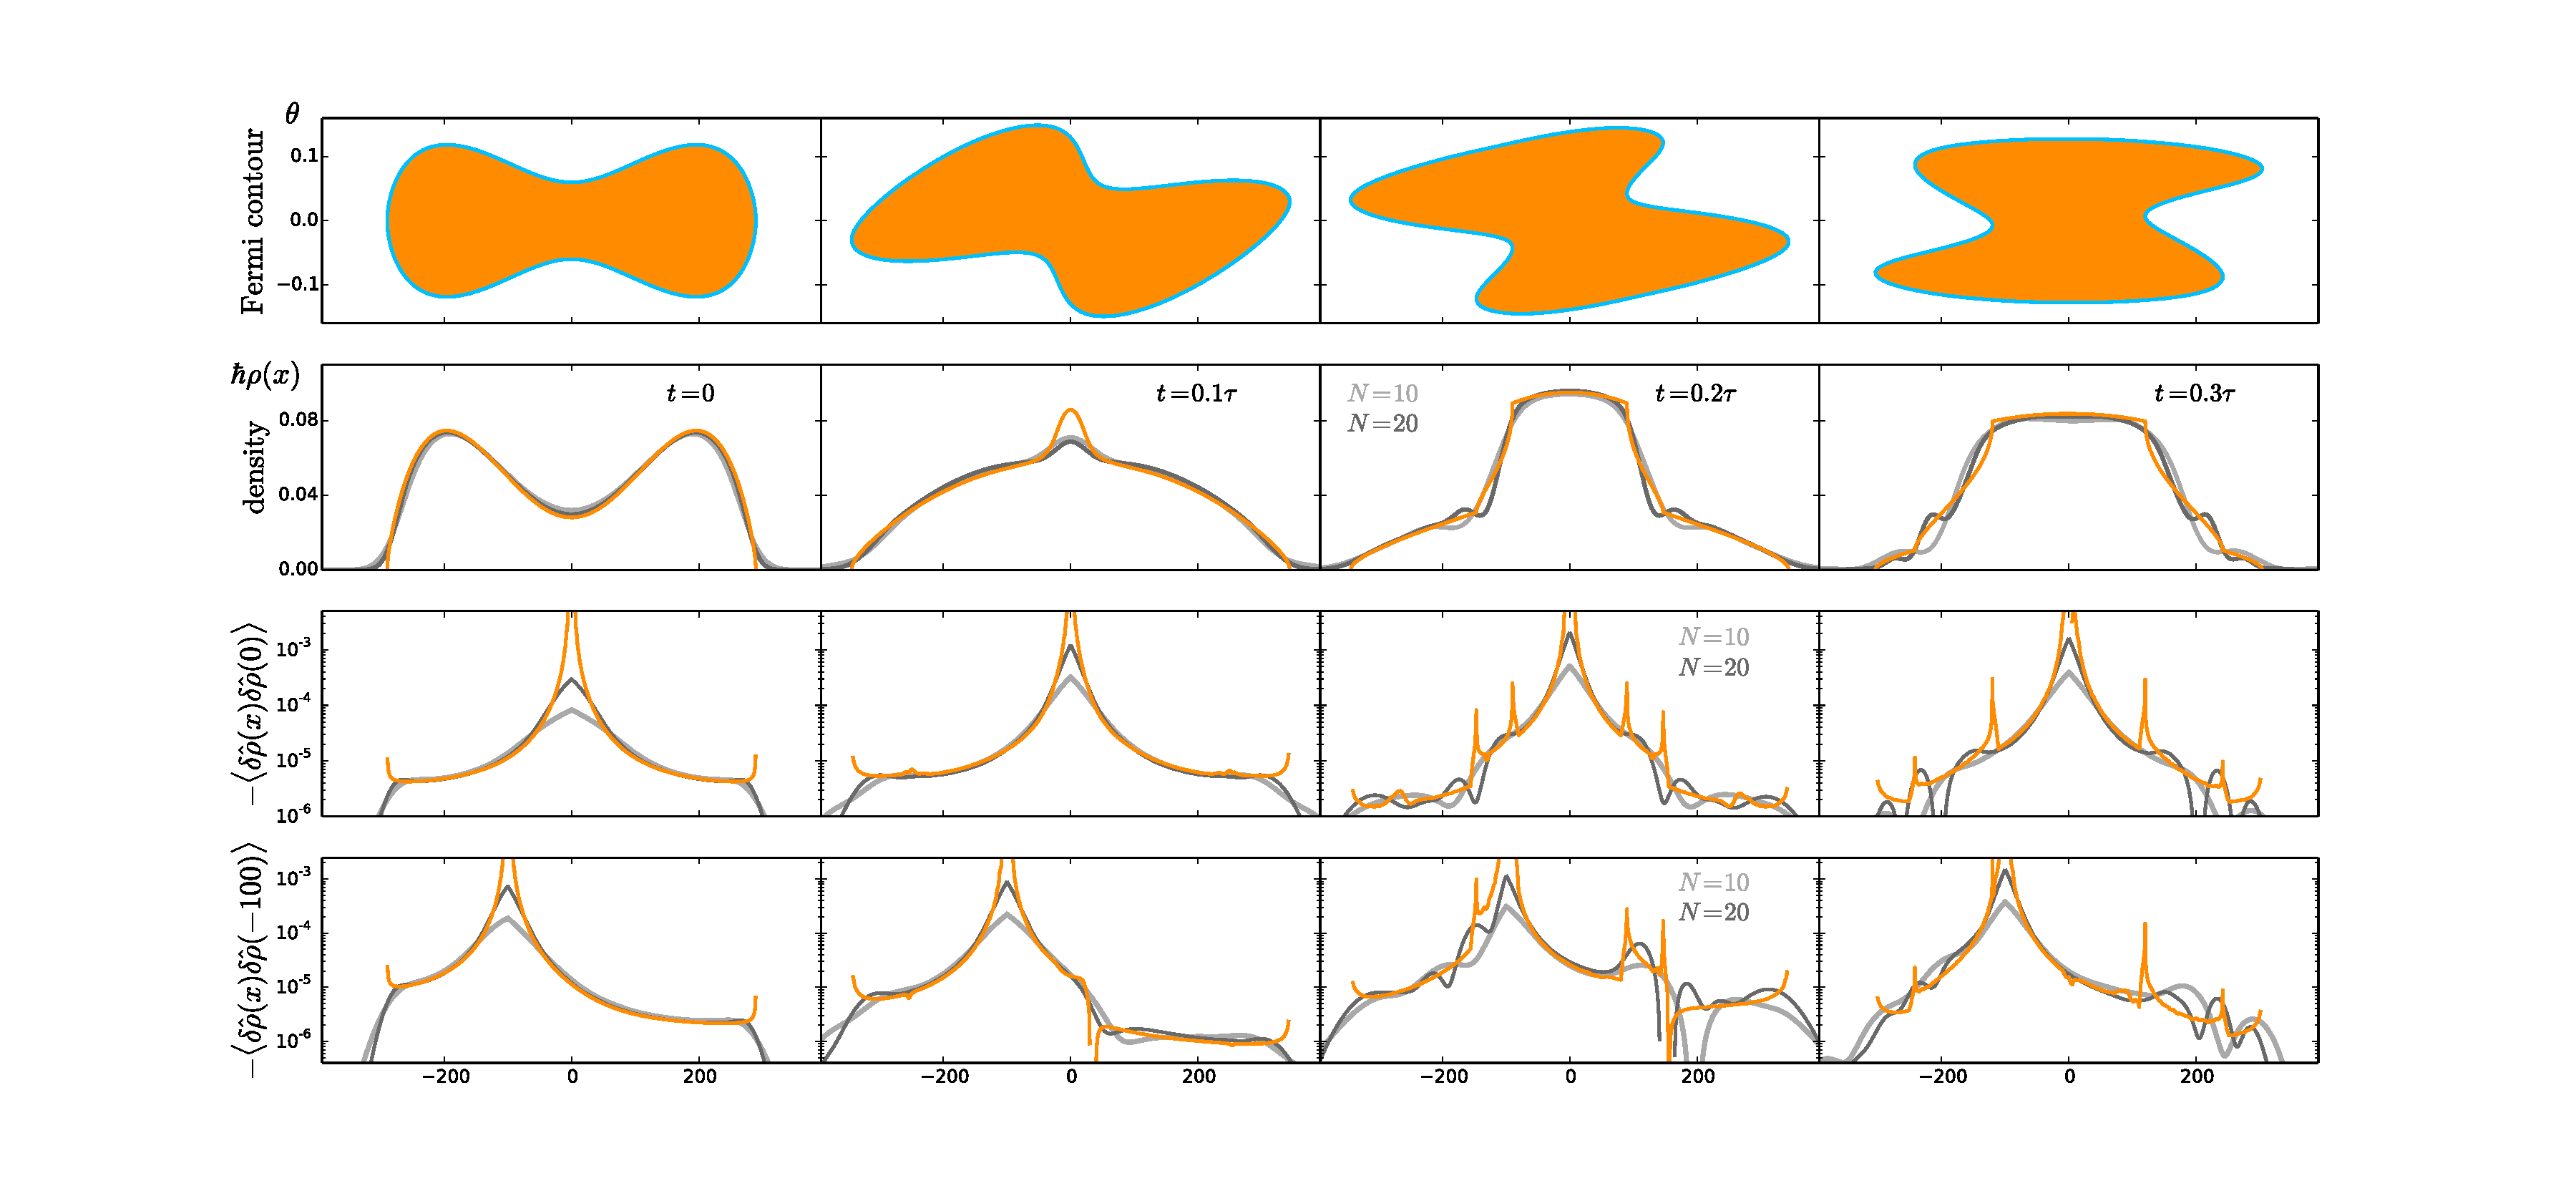
\includegraphics[width = 0.99\textwidth]{fig2.pdf}
\caption{Quantum quench from double to single well in the 1d Bose gas with delta repulsion. We compare the predictions of GHD and QGHD (orange curves) to time-dependent DMRG simulation for N=10 (light gray) and N=20 particles (dark gray). First row: Fermi contour evolved with GHD. Second row: density profile predicted by GHD, compared with DMRG. Third and fourth row: connected density-density correlator $\left< \hat{\rho} (x) \hat{\rho} (x_0)\right>$ predicted by QGHD and compared with DMRG, for two different positions $x_0$. Each row shows the corresponding quantity as a function of the spatial coordinate $x$, at different times, expressed as a fraction of the period $\tau$ (from $t=0$ in the first column to $t=0.3 \tau$ in the last). 
For the DMRG simulation we work with particles on a lattice at very low density. The parameters are: repulsion strength $\bar{g} = 0.1$; $L=800$ lattice sites; number of particles $N=10, 20$; $\hbar = 30/N$; pre-quench potential $V_0(x)= (x/L)^4 - 0.12 (x/L)^2$; post-quench potential $V(x) = \omega^2 x^2 /2$ with $\omega=0.3/L$ (and period $\tau= 2\pi/\omega$). The dimensionless Lieb parameter $\gamma = \frac{\bar{g}}{\hbar \rho}$ is of order $1$, so we are far from both the Gross-Pitaevski limit and the Tonks-Girardeau limit.
\trad{Quantum quench du double puits au puits unique dans le gaz de Bose unidimensionnel avec répulsion delta. Nous comparons les prédictions de la GHD et de la QGHD (courbes orange) à la simulation DMRG dépendante du temps pour N=10 (gris clair) et N=20 particules (gris foncé). Première rangée : contour de Fermi évolué avec la GHD. Deuxième rangée : profil de densité prédit par la GHD, comparé avec DMRG. Troisième et quatrième rangée : fonction de corrélation densité-densité connectée $\left< \hat{\rho} (x) \hat{\rho} (x_0)\right>$ prédite par la QGHD et comparée avec DMRG, pour deux positions différentes $x_0$. Chaque rangée montre la quantité correspondante en fonction de la coordonnée spatiale $x$, à différents moments, exprimés comme une fraction de la période $\tau$ (de $t=0$ dans la première colonne à $t=0.3 \tau$ dans la dernière). 
Pour la simulation DMRG, nous travaillons avec des particules sur un réseau à très faible densité. Les paramètres sont : force de répulsion $\bar{g} = 0.1$ ; $L=800$ sites du réseau ; nombre de particules $N=10, 20$ ; $\hbar = 30/N$ ; potentiel avant la quench $V_0(x)= (x/L)^4 - 0.12 (x/L)^2$ ; potentiel après la quench $V(x) = \omega^2 x^2 /2$ avec $\omega=0.3/L$ (et période $\tau= 2\pi/\omega$). Le paramètre de Lieb adimensionnel $\gamma = \frac{\bar{g}}{\hbar \rho}$ est de l'ordre de $1$, donc nous sommes loin à la fois de la limite de Gross-Pitaevski et de la limite de Tonks-Girardeau.}
}
\label{movie}
\end{figure*}



\vspace{0.1cm} \noindent {\bf\em Quantization of sound waves.}\; The conserved modes $\delta p_a$ can now be given quantum fluctuations, $\delta p_a\rightarrow \delta\hat p_a$. In quantized fluid theory one assumes that there is a classical hydrodynamic action $S = S(\{p_a\})$, whose minimum gives rise to the fluid equation, and which provides the quantum fluctuations and long-range correlations simply by quadratic expansion:
\begin{equation}
	e^{iS} \approx e^{iS_{\rm classical} + i\sum_{ab} S^{(2)}_{ab} \delta p_a \delta p_{b} }.
\end{equation}
Passing to the Hamiltonian formalism, there must be a symplectic structure and a Hamiltonian, quadratic in hydrodynamic wave operators $\delta \hat k_a=\delta \hat p_a/\hbar$, which reproduces \eqref{eq:deltaka}.


To identify those, consider the measure $d p = 1^{\rm dr} d\theta$, which takes into account the density of allowed states $1^{\rm dr}$ \cite{korepin1997quantum}, and the phase-space volume form it induces, $dx \wedge dp = 1^{\rm dr}\, dx \wedge d\theta$. This volume form is preserved by GHD~\cite{doyon2018geometric}. Therefore, the fluctuations at zero entropy are fluctuations of an incompressible region in the $(x,p)$ plane. A first consequence is that small volume variations $d p^a = \sigma_a dp_a$, where $\sigma_a = (-1)^a$ is the chirality of the volume boundary, are thermodynamic potentials, leading to an Onsager reciprocity relation (see SM \cite{SM})
\begin{equation}\label{eq:Asym}
	\mathsf A^{ab} = \mathsf A^{ba} \quad
	(\mathsf A^{ab} = \partial \epsilon_a / \partial k^b
	=\sigma_b \mathsf A_a^{~b}).
\end{equation}
That is, the diagonal matrix $\sigma = {\rm diag}( \{ \sigma_a \}_{1\leq a \leq 2q})$ gives a symplectic structure under which the flux Jacobian is symmetric. Second, the problem of quantizing fluctuations of incompressible regions is well known in the literature on the quantum Hall effect~\cite{wen1990chiral,wen1992theory,iso1992fermions,cappelli1993infinite}. Parameterizing the boundary of that region as $(x(s), p(s))$ and introducing a density operator which measures the excess number of occupied states around $(x(s), p(s))$, $\delta \hat{\rho} (s) = \frac{1}{2\pi \hbar} \frac{dx}{ds}  \delta \hat{p} (x)$, the commutation relation is the one of a chiral U(1) current algebra,
\begin{subequations}
\begin{equation}
	\label{eq:comm_rho}
	\left[ \delta \hat{\rho} (s) ,   \delta \hat{\rho} (s') \right] \, = \, \frac{1}{2\pi i}   \, \delta' (s-s') .
\end{equation}
Equivalently, with the local parameterization $\delta \hat{p}_a(x)$,
\begin{equation}
	\label{eq:comm_p}
	\left[ \delta \hat{p}_a (x) ,   \delta \hat{p}_b (y) \right] \, = \, -i \sigma_a  2\pi \hbar^2   \delta_{ab}  \, \delta' (x-y) .
\end{equation}
\end{subequations}
Using this symplectic structure, the Hamiltonian generating \eqref{eq:deltaka} can be taken as
\begin{equation}
	\label{eq:hamiltonian}
	\hat H[{\Gamma_t}] \,=\,  \frac{1}{4 \pi \hbar} \int dx  \sum_{a,b}   \delta \hat p_a(x) \mathsf A^{ab} \delta \hat p_b(x)  .
\end{equation}
Indeed, together with the commutation relation (\ref{eq:comm_p}), the Heisenberg equation
\begin{equation}
	\frac{d}{dt} \delta \hat p_a (x) = \frac{i}{\hbar} [\hat H[\Gamma_t], \delta \hat p_a (x) ] 
\end{equation}
reproduces the equation for sound waves (\ref{eq:deltaka}).


The dependence of $\hat H[\Gamma_t]$ on $\Gamma_t$ is via that of $\mathsf A^{ab}$ on the Fermi points $\{\theta_c(x,t)\}$. The contour-dependent Hamiltonian (\ref{eq:hamiltonian}) is the most important result of this Letter, and we refer to it as the {\it QGHD Hamiltonian}. Crucially, QGHD is a {\it quadratic theory}, so correlation functions can be calculated easily, at least numerically. [Higher-derivative and higher-order terms would lead to a generalization of the non-linear Luttinger liquid~\cite{imambekov2012one,imambekov2009universal} or nonlinear bosonization~\cite{abanov2005quantum,bettelheim2008quantum,stone2008classical,kulkarni2009nonlinear}; they are beyond the scope of this Letter.]

QGHD is the theory of a multi-component, spatially inhomogeneous, time-dependent, quantum fluctuating liquid with (locally) $q$ coupled components. Importantly, in the particular case of homogeneous time-independent split Fermi seas, we have checked~(see SM \cite{SM}) that it coincides with the multi-component quadratic Hamiltonian of Eli\"ens and Caux~\cite{eliens2016general,eliens2017quantum} (see also Refs.~\cite{fokkema2014split,vlijm2016correlations}). As noted by these authors, the case of a single component $q=1$ is nothing but the standard Luttinger liquid theory.
\trad{\vspace{0.1cm} \noindent {\bf\em Quantification des ondes sonores.}\; Les modes conservés $\delta p_a$ peuvent maintenant être quantifiés, $\delta p_a\rightarrow \delta\hat p_a$. Dans la théorie des fluides quantifiés, on suppose qu'il existe une action hydrodynamique classique $S = S(\{p_a\})$, dont le minimum donne lieu à l'équation du fluide, et qui fournit les fluctuations quantiques et les corrélations à longue portée simplement par une expansion quadratique :
\begin{equation*}
	e^{iS} \approx e^{iS_{\rm classique} + i\sum_{ab} S^{(2)}_{ab} \delta p_a \delta p_{b} }.
\end{equation*}
En passant au formalisme hamiltonien, il doit exister une structure symplectique et un Hamiltonien, quadratique en opérateurs d'onde hydrodynamiques $\delta \hat k_a=\delta \hat p_a/\hbar$, qui reproduit \eqref{eq:deltaka}.
Pour les identifier, considérons la mesure $d p = 1^{\rm dr} d\theta$, qui prend en compte la densité des états autorisés $1^{\rm dr}$ \cite{korepin1997quantum}, et la forme de volume dans l'espace des phases qu'elle induit, $dx \wedge dp = 1^{\rm dr}\, dx \wedge d\theta$. Cette forme de volume est conservée par la GHD~\cite{doyon2018geometric}. Par conséquent, les fluctuations à entropie nulle sont des fluctuations d'une région incompressible dans le plan $(x,p)$. Une première conséquence est que les petites variations de volume $d p^a = \sigma_a dp_a$, où $\sigma_a = (-1)^a$ est la chiralité de la frontière de volume, sont des potentiels thermodynamiques, conduisant à une relation de réciprocité d'Onsager (voir SM \cite{SM})
\begin{equation*}%\label{eq:Asym}
	\mathsf A^{ab} = \mathsf A^{ba} \quad
	(\mathsf A^{ab} = \partial \epsilon_a / \partial k^b
	=\sigma_b \mathsf A_a^{~b}).
\end{equation*}
C'est-à-dire que la matrice diagonale $\sigma = {\rm diag}( \{ \sigma_a \}_{1\leq a \leq 2q})$ donne une structure symplectique sous laquelle le jacobien de flux est symétrique. Deuxièmement, le problème de la quantification des fluctuations des régions incompressibles est bien connu dans la littérature sur l'effet Hall quantique~\cite{wen1990chiral,wen1992theory,iso1992fermions,cappelli1993infinite}. En paramétrant la frontière de cette région comme $(x(s), p(s))$ et en introduisant un opérateur de densité qui mesure le nombre excédentaire d'états occupés autour de $(x(s), p(s))$, $\delta \hat{\rho} (s) = \frac{1}{2\pi \hbar} \frac{dx}{ds}  \delta \hat{p} (x)$, la relation de commutation est celle d'une algèbre de courants U(1) chirale,
\begin{subequations}
\begin{equation*}
	%\label{eq:comm_rho}
	\left[ \delta \hat{\rho} (s) ,   \delta \hat{\rho} (s') \right] \, = \, \frac{1}{2\pi i}   \, \delta' (s-s') .
\end{equation*}
Équivalemment, avec la paramétrisation locale $\delta \hat{p}_a(x)$,
\begin{equation*}
	%\label{eq:comm_p}
	\left[ \delta \hat{p}_a (x) ,   \delta \hat{p}_b (y) \right] \, = \, -i \sigma_a  2\pi \hbar^2   \delta_{ab}  \, \delta' (x-y) .
\end{equation*}
\end{subequations}
En utilisant cette structure symplectique, l'Hamiltonien générant \eqref{eq:deltaka} peut être pris comme
\begin{equation*}
	%\label{eq:hamiltonian}
	\hat H[{\Gamma_t}] \,=\,  \frac{1}{4 \pi \hbar} \int dx  \sum_{a,b}   \delta \hat p_a(x) \mathsf A^{ab} \delta \hat p_b(x)  .
\end{equation*}
En effet, avec la relation de commutation (\ref{eq:comm_p}), l'équation de Heisenberg
\begin{equation*}
	\frac{d}{dt} \delta \hat p_a (x) = \frac{i}{\hbar} [\hat H[\Gamma_t], \delta \hat p_a (x) ] 
\end{equation*}
reproduit l'équation pour les ondes sonores (\ref{eq:deltaka}).
La dépendance de $\hat H[\Gamma_t]$ sur $\Gamma_t$ se fait via celle de $\mathsf A^{ab}$ sur les points de Fermi $\{\theta_c(x,t)\}$. L'Hamiltonien dépendant du contour (\ref{eq:hamiltonian}) est le résultat le plus important de cette Lettre, et nous le désignons comme l' {\it Hamiltonien QGHD}. De manière cruciale, la QGHD est une {\it théorie quadratique}, de sorte que les fonctions de corrélation peuvent être calculées facilement, du moins numériquement. [Les termes d'ordre supérieur et les dérivées d'ordre supérieur conduiraient à une généralisation du liquide de Luttinger non linéaire~\cite{imambekov2012one,imambekov2009universal} ou à une bosonisation non linéaire~\cite{abanov2005quantum,bettelheim2008quantum,stone2008classical,kulkarni2009nonlinear}; ils sont au-delà du champ de cette Lettre.]
La QGHD est la théorie d'un liquide quantique fluctuants multi-composants, spatialement inhomogène, dépendant du temps, avec des composants couplés (localement) $q$. Il est important de noter que dans le cas particulier des mers de Fermi divisées homogènes et indépendantes du temps, nous avons vérifié~(voir SM \cite{SM}) que cela coïncide avec l'Hamiltonien quadratique multi-composants d'Eli\"ens et Caux~\cite{eliens2016general,eliens2017quantum} (voir aussi Refs.~\cite{fokkema2014split,vlijm2016correlations}). Comme l'ont noté ces auteurs, le cas d'un seul composant $q=1$ n'est autre que la théorie standard du liquide de Luttinger.
}



\vspace{0.1cm}
\noindent {\bf\em An example, and numerical check.}\; To illustrate the possibilities offered by QGHD, we consider the dynamics of the 1d Bose gas after a quench of the trapping potential from double-well, $V_0(x)= a_4 x^4 - a_2 x^2$, to harmonic, $V(x) = \omega^2 x^2/2$. The gas is initially in its ground state in $V_0(x)$, with a single pair of Fermi points (i.e. $q=1$) everywhere. At time $t>0$, after some fraction of the period of the trap $\tau = \frac{2\pi}{\omega}$, the contour $\Gamma_t$ gets deformed and a region appears near the boundaries with a split Fermi sea $q=2$. Hence this is a true out-of-equilibrium situation, not describable by standard hydrodynamics. This protocol mimics the famous quantum Newton's cradle~\cite{kinoshita2006quantum} and it can be realized experimentally (see e.g. Refs.~\cite{schemmer2019generalized,joseph2011observation}).



We focus on the equal-time density-density correlation function (Fig.~\ref{movie}). At a point $x$, the fluctuations of the particle density are measured by the operator 
\begin{equation}
	\delta \hat{\rho} (x,t) \, = \, \sum_s  \left| \frac{ds}{dx} \right| \delta \hat{\rho} (s) \, = \, \sum_{a}  \frac{1}{2\pi \hbar} \delta \hat{p}_a ,
\end{equation}
which is a sum over the $2q$ Fermi points at $(x,t)$. Its two-point function at time $t$ is
\begin{eqnarray} \label{rhorho}
	\left< \delta \hat{\rho} (x,t) \delta \hat{\rho} (x',t) \right>  &=&  \sum_{s} \sum_{s'} \left| \frac{ds}{dx} \right|  \left| \frac{ds'}{dx'} \right| G((s,t),(s',t)) , \nonumber\quad
\end{eqnarray}
where $ G((s,t),(s',t'))$ is the Green's function along the contour $G((s,t) ,(s' ,t')) \, = \, \left< \delta \hat{\rho} (s,t) \delta \hat{\rho} (s',t') \right>$. At $t=t'=0$, $G((s,0),(s',0))$ is the ground state correlation in the Hamiltonian $\hat{H}[\Gamma_0]$. At later times $G((s,t),(s',t'))$ satisfies the evolution equation derived from
\begin{equation}
	\frac{d}{dt} \delta \hat{\rho} (s,t) \, = \, \partial_s (v(s) \delta \hat{\rho} (s,t)) + \frac{i}{\hbar} [ \hat{H} [\Gamma_t], \delta \hat{\rho}(s,t) ] ,
\end{equation}
where $v(s) = v^{\rm eff} (\theta_a) \frac{dx}{ds}$ if $a$ labels the local Fermi point with parameter $s$. Importantly, $G((s,t),(s',t'))$ is of order $O(1)$ in the limit (\ref{eq:limit}), so we see that QGHD captures the first correction to the classical result (which is zero):
\begin{eqnarray}
	\frac{ \left< \delta \hat{\rho} (x,t) \delta \hat{\rho} (x',t) \right> }{\rho_{\rm cl.} (x) \rho_{\rm cl.} (x') 
} = O(\hbar^2) .
\end{eqnarray}



In Fig.~\ref{movie} we numerically evaluate the Green's function and compare the QGHD prediction (\ref{rhorho}) with a time-dependent Density-Matrix Renormalization Group (tDRMG)~\cite{dmrg-rev, itensor} simulation of the microscopic model. The dimensionless Lieb parameter $\gamma = \frac{\bar{g}}{\hbar \rho}$ is chosen to be of order $1$, so we are in the truly interacting regime of the 1d Bose gas, away from both the 
Gross-Pitaevski and the Tonks-Girardeau limits. 
The tDMRG simulation is performed for a lattice gas at very low density ($N \ll L$, where $L$ is the number of lattice sites)~\cite{schmidt2007exact,peotta2014quantum}, to be as close as possible to the continuum limit.
The largest number of particles accessible with this method is of order of $N \sim 20$~\cite{peotta2014quantum}, hence far from the thermodynamic limit. Consequently, finite-$N$ effects are large in our data, which we display for $N = 10, 20$ (and $L =800$). Still, the agreement between QGHD and numerics is good, and it improves as $\hbar$ decreases (i.e. $N\sim 1/\hbar$ increases). The tDMRG simulation becomes less accurate at large time; for this reason we stop the simulation at $t= 0.3 \tau$.
The limitations of tDMRG to small $N$ and small $t$ make the predictive power of QGHD even more apparent: QGHD does not suffer from those limitations as it works directly in the thermodynamic limit.

One interesting physical feature of Fig.~\ref{movie} is the divergence of the density-density correlation, in the thermodynamic limit, at the points where a change in the number of Fermi points occurs. They come from the Jacobians in Eq. (\ref{rhorho}) and are genuine predictions of the theory, valid for large enough $N$. The presence of these peaks can be explicitly confirmed by direct computations in the Tonks-Girardeau limit, where they are superimposed to Friedel oscillations~\cite{inpreparation} (see also Ref.~\cite{brun2018inhomogeneous} about the equilibrium case in a trap, where these divergences appear near the edges of the system), but they are a general consequence of QGHD at any interaction strength. At the small value $N=20$, the peaks' extent is smaller than that of Euler fluid cells, hence the peaks are washed away, as seen in the tDMRG result of Fig.~\ref{movie}.

% At $N=20$, however, the peaks' extent is smaller than that of Euler fluid cells, hence the peaks are washed away. Crucially, though, as is apparent in Fig.~\ref{movie}, even for such a small number of particles, the smooth part of the QGHD prediction remains quite accurate, because it is on large enough scales. This interpretation is confirmed in more details in the Tonks-Girardeau limit~\cite{inpreparation}.}




%To obtain this numerical solution, we focus on the Tonks-Girardeau (TG) limit $\bar{g} \rightarrow \infty$, where standard free fermion techniques apply~\cite{girardeau1960relationship} and give access to numerical results for large numbers of particles and long times. Because we focus on the TG limit, some simplifications occur also on the analytical side. In particular, the equation for sound waves is simply $\frac{d}{dt} \delta \hat{\rho}(s ,t ) = 0$, reflecting the underlying non-interacting fermion dynamics. Moreover the hamiltonian \eqref{eq:hamiltonian} is the one of a system with underlying conformal invariance in a fictitious curved space-time encoding the inhomogeneity~\cite{dubail2017conformal,brun2017one,ruggiero2019conformal}. These simplifications allow to obtain the Green's function along the contour in an analytically closed form. Indeed, chosing the $s$-parameterization of the initial contour $\Gamma_0$ such that $(d x_0(s), d p_0(s)) \propto ( p_0(x_0(s)) ds, \frac{d p_0(x)}{x} \frac{dx_0}{ds} ds )$ with $p_0(x) = \sqrt{2 (\mu - V_0 (x))}$, the Green's function turns out to be simply~\cite{dubail2017conformal,ruggiero2019conformal} $G ((s,t) ,(s',t)) = - \ln \left( 2 \sin ( (s-s')/2)\right)$, independently of $t$. Plugging this into Eq.~(\ref{rhorho}), one gets the result plotted in the third row of Fig.~\ref{movie}. The exact microscopic solution has large Friedel oscillations (cyan curve), which we cancel by spatially averaging over a small window $[x-\Delta x/2,x+\Delta x/2]$. After averaging, the agreement with the prediction of QGHD is remarkable.

%We also study the entanglement entropy, which vanishes in GHD \cite{entGHDfree,entGHDint}, but is non-zero in QGHD. The entanglement entropy is particularly challenging to compute directly within the microscopic model and therefore its calculation manifests the predictive power of our approach. It is defined as $S(x,t) = - \textrm{tr} \sigma_A \log \sigma_A$, in terms of the reduced density matrix $\sigma_A$. We focus on the subsystem $A= [-\infty, x]$.
%In the SM~\cite{SM} we show that $S(x, t)$ can be obtained ---via replica approach--- from either a two-point or a four-point correlation function 
%(depending on the number of Fermi points at $(x, t)$) of a special scaling operator of the chiral theory.
%The comparison with numerics is shown in the last row of Fig.~\ref{movie}: the agreement is impressive.

\trad{\vspace{0.1cm}
\noindent {\bf\em Un exemple et vérification numérique.}\; Pour illustrer les possibilités offertes par la QGHD, nous considérons la dynamique du gaz de Bose 1D après un quench du potentiel de piégeage d'un puits double, $V_0(x)= a_4 x^4 - a_2 x^2$, à un potentiel harmonique, $V(x) = \omega^2 x^2/2$. Le gaz est initialement dans son état fondamental dans $V_0(x)$, avec une seule paire de points de Fermi (i.e. $q=1$) partout. Au temps $t>0$, après une fraction du période du piège $\tau = \frac{2\pi}{\omega}$, le contour $\Gamma_t$ se déforme et une région apparaît près des frontières avec une mer de Fermi éclatée $q=2$. Il s'agit donc d'une véritable situation hors d'équilibre, non décrite par l'hydrodynamique standard. Ce protocole imite le célèbre pendule de Newton quantique~\cite{kinoshita2006quantum} et peut être réalisé expérimentalement (voir par exemple Refs.~\cite{schemmer2019generalized,joseph2011observation}).
Nous nous concentrons sur la fonction de corrélation densité-densité à temps égal (Fig.~\ref{movie}). En un point $x$, les fluctuations de la densité de particules sont mesurées par l'opérateur 
\begin{equation*}
	\delta \hat{\rho} (x,t) \, = \, \sum_s  \left| \frac{ds}{dx} \right| \delta \hat{\rho} (s) \, = \, \sum_{a}  \frac{1}{2\pi \hbar} \delta \hat{p}_a ,
\end{equation*}
qui est une somme sur les $2q$ points de Fermi en $(x,t)$. Sa fonction à deux points au temps $t$ est
\begin{eqnarray*} %\label{rhorho}
	\left< \delta \hat{\rho} (x,t) \delta \hat{\rho} (x',t) \right>  &=&  \sum_{s} \sum_{s'} \left| \frac{ds}{dx} \right|  \left| \frac{ds'}{dx'} \right| G((s,t),(s',t)) , \nonumber\quad
\end{eqnarray*}
où $ G((s,t),(s',t'))$ est la fonction de Green le long du contour $G((s,t) ,(s' ,t')) \, = \, \left< \delta \hat{\rho} (s,t) \delta \hat{\rho} (s',t') \right>$. À $t=t'=0$, $G((s,0),(s',0))$ est la corrélation dans l'état fondamental de l'Hamiltonien $\hat{H}[\Gamma_0]$. À des temps ultérieurs, $G((s,t),(s',t'))$ satisfait l'équation d'évolution dérivée de
\begin{equation*}
	\frac{d}{dt} \delta \hat{\rho} (s,t) \, = \, \partial_s (v(s) \delta \hat{\rho} (s,t)) + \frac{i}{\hbar} [ \hat{H} [\Gamma_t], \delta \hat{\rho}(s,t) ] ,
\end{equation*}
où $v(s) = v^{\rm eff} (\theta_a) \frac{dx}{ds}$ si $a$ étiquette le point de Fermi local avec le paramètre $s$. Il est important de noter que $G((s,t),(s',t'))$ est de l'ordre $O(1)$ dans la limite (\ref{eq:limit}), donc nous voyons que la QGHD capture la première correction au résultat classique (qui est nul) :
\begin{eqnarray*}
	\frac{ \left< \delta \hat{\rho} (x,t) \delta \hat{\rho} (x',t) \right> }{\rho_{\rm cl.} (x) \rho_{\rm cl.} (x') 
} = O(\hbar^2) .
\end{eqnarray*}
Dans la Fig.~\ref{movie}, nous évaluons numériquement la fonction de Green et comparons la prédiction de la QGHD (\ref{rhorho}) avec une simulation par la méthode de Renormalisation de Matrice de Densité (tDRMG)~\cite{dmrg-rev, itensor} du modèle microscopique. Le paramètre de Lieb sans dimension $\gamma = \frac{\bar{g}}{\hbar \rho}$ est choisi de l'ordre de $1$, donc nous sommes dans le régime véritablement interactif du gaz de Bose 1D, loin des limites de Gross-Pitaevski et de Tonks-Girardeau. La simulation tDMRG est effectuée pour un gaz sur réseau à très basse densité ($N \ll L$, où $L$ est le nombre de sites du réseau)~\cite{schmidt2007exact,peotta2014quantum}, pour être aussi proche que possible de la limite continue. Le plus grand nombre de particules accessible avec cette méthode est de l'ordre de $N \sim 20$~\cite{peotta2014quantum}, donc loin de la limite thermodynamique. En conséquence, les effets de taille finie sont importants dans nos données, que nous affichons pour $N = 10, 20$ (et $L = 800$). Cependant, l'accord entre la QGHD et les résultats numériques est bon, et il s'améliore à mesure que $\hbar$ diminue (c'est-à-dire que $N\sim 1/\hbar$ augmente). La simulation tDMRG devient moins précise à des temps longs ; pour cette raison, nous arrêtons la simulation à $t= 0.3 \tau$. Les limitations de tDMRG à petits $N$ et petits $t$ rendent le pouvoir prédictif de la QGHD encore plus évident : la QGHD ne souffre pas de ces limitations puisqu'elle fonctionne directement dans la limite thermodynamique.
Une caractéristique physique intéressante de la Fig.~\ref{movie} est la divergence de la corrélation densité-densité, dans la limite thermodynamique, aux points où un changement dans le nombre de points de Fermi se produit. Elles proviennent des Jacobiens dans l'équation (\ref{rhorho}) et sont de véritables prédictions de la théorie, valides pour des $N$ suffisamment grands. La présence de ces pics peut être confirmée explicitement par des calculs directs dans la limite de Tonks-Girardeau, où ils sont superposés aux oscillations de Friedel~\cite{inpreparation} (voir aussi Ref.~\cite{brun2018inhomogeneous} concernant le cas d'équilibre dans un piège, où ces divergences apparaissent près des bords du système), mais elles sont une conséquence générale de la QGHD pour toute force d'interaction. À la petite valeur $N=20$, l'étendue des pics est plus petite que celle des cellules de fluide d'Euler, donc les pics sont atténués, comme on le voit dans le résultat tDMRG de la Fig.~\ref{movie}.\\
(en cache !!!!) \\
À $N=20$, cependant, l'étendue des pics est plus petite que celle des cellules de fluide d'Euler, donc les pics sont atténués. De manière cruciale, toutefois, comme il est évident dans la Fig.~\ref{movie}, même pour un si petit nombre de particules, la partie lisse de la prédiction de la QGHD reste assez précise, car elle est à des échelles suffisamment grandes. Cette interprétation est confirmée plus en détails dans la limite de Tonks-Girardeau~\cite{inpreparation}. 
Pour obtenir cette solution numérique, nous nous concentrons sur la limite de Tonks-Girardeau (TG) $\bar{g} \rightarrow \infty$, où les techniques de fermions libres standard s'appliquent~\cite{girardeau1960relationship} et donnent accès à des résultats numériques pour un grand nombre de particules et de longs temps. Parce que nous nous concentrons sur la limite TG, certaines simplifications se produisent également du côté analytique. En particulier, l'équation pour les ondes sonores est simplement $\frac{d}{dt} \delta \hat{\rho}(s ,t ) = 0$, reflétant la dynamique de fermions non-interagissants sous-jacente. De plus, l'hamiltonien \eqref{eq:hamiltonian} est celui d'un système avec invariance conforme sous-jacente dans un espace-temps courbé fictif encodant l'inhomogénéité~\cite{dubail2017conformal,brun2017one,ruggiero2019conformal}. Ces simplifications permettent d'obtenir la fonction de Green le long du contour sous une forme analytique fermée. En effet, en choisissant la paramétrisation $s$ du contour initial $\Gamma_0$ de sorte que $(d x_0(s), d p_0(s)) \propto ( p_0(x_0(s)) ds, \frac{d p_0(x)}{x} \frac{dx_0}{ds} ds )$ avec $p_0(x) = \sqrt{2 (\mu - V_0 (x))}$, la fonction de Green est simplement~\cite{dubail2017conformal,ruggiero2019conformal} $G ((s,t) ,(s',t)) = - \ln \left( 2 \sin ( (s-s')/2)\right)$, indépendamment de $t$. En insérant cela dans l'équation (\ref{rhorho}), on obtient le résultat tracé dans la troisième rangée de la Fig.~\ref{movie}. La solution microscopique exacte a de grandes oscillations de Friedel (courbe cyan), que nous annulons en moyennant spatialement sur une petite fenêtre $[x-\Delta x/2,x+\Delta x/2]$. Après moyenne, l'accord avec la prédiction de la QGHD est remarquable.
Nous étudions également l'entropie de von Neumann, qui est nulle dans la GHD \cite{entGHDfree,entGHDint}, mais non nulle dans la QGHD. L'entropie de von Neumann est particulièrement difficile à calculer directement dans le modèle microscopique et donc son calcul manifeste le pouvoir prédictif de notre approche. Elle est définie comme $S(x,t) = - \textrm{tr} \sigma_A \log \sigma_A$, en termes de la matrice de densité réduite $\sigma_A$. Nous nous concentrons sur le sous-système $A= [-\infty, x]$. Dans le SM~\cite{SM}, nous montrons que $S(x, t)$ peut être obtenu ---via une approche de réplicas--- à partir soit d'une fonction de corrélation à deux points soit à quatre points 
(en fonction du nombre de points de Fermi en $(x, t)$) d'un opérateur de mise à l'échelle spécial de la théorie chirale.
La comparaison avec les résultats numériques est montrée dans la dernière rangée de la Fig.~\ref{movie} : l'accord est impressionnant.
}




\vspace{0.1cm}
\noindent {\bf\em Conclusion.}\; By focusing on the GHD description of the integrable 1d Bose gas in states of zero entropy, we showed that quantum effects which fall beyond the GHD description can be reconstructed by allowing quantum fluctuations of the Fermi contour.
We have been partially inspired by linear fluctuating hydrodynamics \cite{abanov2006hydrodynamics,spohn2014nlfh}, where
fluctuations are accessed by phenomenologically adding thermal noise to the linear response evolution of conserved fluid modes.
We follow the general principles of this theory, but instead of adding thermal noise, we use ideas from quantum fluids
(see e.g. \cite{abanov2006hydrodynamics}) in order to access quantum fluctuations.
To benchmark QGHD, we applied it to a zero entropy quench in the 1d Bose gas, providing exact predictions for the equal time density-density correlations, and checking that they are in good agreement with numerical tDMRG data obtainable for a small particle number and short times.

%This new theory of QGHD opens up a plethora of fundamental applications, mainly, but not only, to those non-equilibrium situations with zero entropy states, where standard GHD provides vanishing (or trivial) predictions for most observables. Among these, we mention the domain wall quench in spin chains \cite{,dubail2017conformal,collura2018analytic}, some local and geometric quenches \cite{localquench1,localquench2,geomquench}, the true quantum Newton cradle protocol \cite{kinoshita2006quantum}, and many more. Some further generalizations of the theory, such as to include non-linear effects (see \cite{abanov2006hydrodynamics} for the equilibrium counterpart), may provide insights on (sub-, super-)diffusion in one-dimensional quantum transport.


%for an interaction parameter away from free boson and fermion limits.
%Other relevant examples are the ripples of the density profile and
%bosonic correlations functions.
%Our approach applies to interacting integrable models as well: we focused on the non-interacting limit for sake of clarity, but results for
%the interacting models will be presented in a more technical follow up \cite{longversion}.
%This new theory of QGHD opens up a plethora of fundamental applications, mainly, but not only, to those non-equilibrium situations with zero entropy states, where standard GHD provides vanishing (or trivial) predictions for most observables. Among these, we mention the domain wall quench in spin chains \cite{,dubail2017conformal,collura2018analytic}, some local and geometric quenches \cite{localquench1,localquench2,geomquench}, the true quantum Newton cradle protocol \cite{kinoshita2006quantum}, and many more. Some further generalizations of the theory, such as to include non-linear effects (see \cite{abanov2006hydrodynamics} for the equilibrium counterpart), may provide insights on (sub-, super-)diffusion in one-dimensional quantum transport.

\trad{\vspace{0.1cm}
\noindent {\bf\em Conclusion.}\; En se concentrant sur la description GHD du gaz de Bose 1D intégrable dans des états de zéro entropie, nous avons montré que les effets quantiques qui échappent à la description GHD peuvent être reconstruits en permettant les fluctuations quantiques du contour de Fermi. Nous avons été partiellement inspirés par l'hydrodynamique linéaire fluctuante \cite{abanov2006hydrodynamics,spohn2014nlfh}, où les fluctuations sont accessibles en ajoutant de manière phénoménologique du bruit thermique à l'évolution en réponse linéaire des modes fluides conservés. Nous suivons les principes généraux de cette théorie, mais au lieu d'ajouter du bruit thermique, nous utilisons des idées provenant des fluides quantiques (voir par exemple \cite{abanov2006hydrodynamics}) afin d'accéder aux fluctuations quantiques. Pour évaluer la QGHD, nous l'avons appliquée à un quench à zéro entropie dans le gaz de Bose 1D, fournissant des prédictions exactes pour les corrélations densité-densité à temps égal, et vérifiant qu'elles sont en bon accord avec les données numériques tDMRG obtenues pour un petit nombre de particules et des temps courts.\\
(en cache !!!) \\
Cette nouvelle théorie de la QGHD ouvre une multitude d'applications fondamentales, principalement, mais pas uniquement, à ces situations hors d'équilibre avec des états de zéro entropie, où la GHD standard fournit des prédictions nulles (ou triviales) pour la plupart des observables. Parmi celles-ci, nous mentionnons le quench de mur de domaine dans les chaînes de spins \cite{,dubail2017conformal,collura2018analytic}, certains quenches locaux et géométriques \cite{localquench1,localquench2,geomquench}, le véritable protocole du pendule de Newton quantique \cite{kinoshita2006quantum}, et bien d'autres. Certaines généralisations ultérieures de la théorie, telles que l'inclusion d'effets non linéaires (voir \cite{abanov2006hydrodynamics} pour le correspondant en équilibre), pourraient fournir des éclaircissements sur la (sous-, sur-) diffusion dans le transport quantique unidimensionnel.
pour un paramètre d'interaction éloigné des limites de bosons et de fermions libres. D'autres exemples pertinents sont les ondulations du profil de densité et les fonctions de corrélations bosoniques. Notre approche s'applique également aux modèles intégrables interactifs : nous nous sommes concentrés sur la limite non-interagissante pour des raisons de clarté, mais les résultats pour les modèles interactifs seront présentés dans un suivi plus technique \cite{longversion}. Cette nouvelle théorie de la QGHD ouvre une multitude d'applications fondamentales, principalement, mais pas uniquement, à ces situations hors d'équilibre avec des états de zéro entropie, où la GHD standard fournit des prédictions nulles (ou triviales) pour la plupart des observables. Parmi celles-ci, nous mentionnons le quench de mur de domaine dans les chaînes de spins \cite{,dubail2017conformal,collura2018analytic}, certains quenches locaux et géométriques \cite{localquench1,localquench2,geomquench}, le véritable protocole du pendule de Newton quantique \cite{kinoshita2006quantum}, et bien d'autres. Certaines généralisations ultérieures de la théorie, telles que l'inclusion d'effets non linéaires (voir \cite{abanov2006hydrodynamics} pour le correspondant en équilibre), pourraient fournir des éclaircissements sur la (sous-, sur-) diffusion dans le transport quantique unidimensionnel.
}

 
\vspace{0.1cm}
\begin{acknowledgments}
We thank S. Eli\"ens, M. Fagotti and J. de Nardis for discussions and A. Bastianello, E. Bettelheim, Y. Brun, A. De Luca, M. Collura, J. Viti and J.-M. St\'ephan for  collaboration on closely related topics. The DMRG simulation in Fig. 2 was done with iTensor~\cite{itensor}; we thank F. Pascale, J.-M. St\' ephan and T. Botzung for help with that simulation. We are grateful to the International Institute of Physics, Natal, Brazil, and to the University of Amsterdam, Netherlands, for hospitality during the completion of this work. Part of this work was supported by the CNRS ``D\'efi Infiniti'' MUSIQ (JD). PC and PR acknowledge support from ERC under Consolidator grant number 771536 (NEMO). BD acknowledges support from Royal Society under Leverhulme Trust Senior Research Fellowship SRF$\setminus$R1$\setminus$180103 ``Emergent hydrodynamics in integrable systems: non-equilibrium theory''; BD is also grateful to the Tokyo Institute of Technology, Tokyo, Japan, for funding and hospitality.
\trad{
Nous remercions S. Eli\"ens, M. Fagotti et J. de Nardis pour les discussions, ainsi que A. Bastianello, E. Bettelheim, Y. Brun, A. De Luca, M. Collura, J. Viti et J.-M. St\'ephan pour leur collaboration sur des sujets étroitement liés. La simulation DMRG présentée dans la Fig. 2 a été réalisée avec iTensor~\cite{itensor} ; nous remercions F. Pascale, J.-M. St\'ephan et T. Botzung pour leur aide avec cette simulation. Nous sommes reconnaissants à l'International Institute of Physics, Natal, Brésil, et à l'Université d'Amsterdam, Pays-Bas, pour leur accueil pendant la réalisation de ce travail. Une partie de ce travail a été soutenue par le CNRS ``Défi Infiniti'' MUSIQ (JD). PC et PR remercient l'ERC pour le soutien apporté sous la subvention Consolidator numéro 771536 (NEMO). BD remercie la Royal Society pour le soutien accordé dans le cadre de la Leverhulme Trust Senior Research Fellowship SRF$\setminus$R1$\setminus$180103 ``Hydrodynamique émergente dans les systèmes intégrables : théorie hors d'équilibre'' ; BD est également reconnaissant envers le Tokyo Institute of Technology, Tokyo, Japon, pour le financement et l'hospitalité.
}
\end{acknowledgments}



\bibliography{qGHD}




\newpage


\begin{widetext}


\begin{center}
{\bf Supplementary material for ``Quantum Generalized Hydrodynamics''}
\end{center}


\section{Details of the derivation of Eq. (7) in the main text}


In this section we derive Eq. (7) in the main text. We start from the GHD equations (4a)-(4b) in the main text. Parametrizing the
contour locally as $\theta_a (x,t)$ and injecting this parametrization into Eq.~(4a), one gets
\begin{eqnarray*}
	\frac{d}{dt} \left( \begin{array}{c}
		x_t(s) \\
		\theta_a (x_t(s), t)
	\end{array} \right) &=& \left(  \begin{array}{c}
		v^{\rm eff} (x_t(s), \theta_a(x_t(s),t) ) \\
		a^{\rm eff} (x_t(s), \theta_a(x_t(s),t) )
	\end{array} \right)  .
\end{eqnarray*}
The second line reads $\partial_t \theta_a (x_t(s), t) + (\partial_t x_t) \partial_x \theta_a (x_t(s), t)  =  a^{\rm eff} (x_t(s), t)$. 
Then, plugging the first line $\partial_t x_t = v^{\rm eff}$ into it, one gets the zero-entropy GHD equation of Ref.~\cite{doyon2017large}:
\begin{equation}
	 \partial_t \theta_a (x, t) + v^{\rm eff}(x,\theta_a)  \partial_x \theta_a (x, t)  = a^{\rm eff} (x,t).
\end{equation}
Finally, we use Eq. (6) in the main text: $\partial_t p  + \partial_x \epsilon + a^{\rm eff} 1^{\rm dr} = 0$. With $p_a = p(\theta_a)$ and $\epsilon_a = \epsilon(\theta_a)$, this gives
\begin{eqnarray*}
	\partial_t p_a + \partial_x \epsilon_a &=&  [ \partial_t p  + \partial_x \epsilon]  (\theta_a) + (\partial_t \theta_a) (\partial_{\theta} p)  + (\partial_x \theta_a)  (\partial_{\theta} \epsilon)  \\
	&=& - a^{\rm eff} (\theta_a) 1^{\rm dr}  (\theta_a)  + (\partial_{\theta} p) \left[ \partial_t \theta_a +  \frac{\partial_{\theta} \epsilon}{\partial_{\theta} p}  \partial_x \theta_a\right] \\
	&=& - a^{\rm eff} (\theta_a) 1^{\rm dr}  (\theta_a)  + (\partial_{\theta} p) \left[ \partial_t \theta_a + v^{\rm eff} (\theta_a) \partial_x \theta_a  \right] \\
	&=&  \left(  - 1^{\rm dr}  (\theta_a)  + \partial_{\theta} p \right) a^{\rm eff} (\theta_a)  .
\end{eqnarray*}
Finally, using the identity $\partial_{\theta} p = ({\rm id}')^{\rm dr} (\theta) = 1^{\rm dr} (\theta) $ ---see Eqs. (\ref{sm:eq:drDr}) and (\ref{sm:eq:k}) in this Supplemental Material---, the last line cancels and one gets $\partial_t p_a + \partial_x \epsilon_a = 0$, which is Eq. (7) in the main text.






\section{Onsager reciprocity relation and consistency with Eli\"ens-Caux formalism}


In this section we expose in full details the Thermodynamic Bethe Ansatz (TBA) calculations that are useful to arrive at the Onsager reciprocity relation (Eq. (10) in the main text) and at the consistency of our results with the ones previously obtained by Eli\"ens and Caux \cite{eliens2016general,eliens2017quantum}.



\subsection{Useful definitions: shift function, ``dressing'' and ``Dressing''}

%The counting function $\rho_{\rm s}(\theta)$ is defined by the constitutive equation, which encodes the Bethe equations in the thermodynamic limit:
%\begin{equation}
%	\label{sm:eq:rhos}
%	\rho_{\rm s} (\theta) \, = \, \frac{1}{2\pi} +  \int_M \frac{d \theta'}{2\pi} \varphi(\theta-\theta') \rho_{\rm s} (\theta') ,
%\end{equation}
The shift function is defined as follows (see e.g. chapter 1 of Ref.~\cite{korepin1997quantum}). Adding a (fermionic) particle with rapidity $\theta$ results in a global shift of all rapidities measured by the shift function
\begin{eqnarray}
	\label{sm:eq:shift}	
F(\theta | \theta') &=& \frac{\phi(\theta-\theta')}{2\pi} + \int_M \frac{d\lambda}{2\pi} \varphi(\theta-\lambda) F(\lambda | \theta') 
%\\&=& 
=	\frac{[\phi(.-\theta')]^{\rm dr} (\theta)}{2\pi} ,
\end{eqnarray}
where $M = [\theta_1,\theta_2] \cup [\theta_3,\theta_4] \cup \dots \cup [\theta_{2n-1},\theta_{2n}]$ is the split Fermi sea. The dressing is the linear operation $f(\theta) \mapsto f^{\rm dr}(\theta)$ defined by the integral equation
\begin{equation}
	\label{sm:eq:dr}
	f^{\rm dr} (\theta) = f(\theta) + \int_M \frac{d\theta'}{2\pi} \varphi(\theta-\theta') f^{\rm dr}(\theta') .
\end{equation}
A very useful property of this dressing operation is that it is symmetric,
\begin{equation}
	\int_M \frac{d\theta}{2\pi} f^{\rm dr} (\theta) g(\theta) \, = \, \int_M \frac{d\theta}{2\pi} f (\theta) g^{\rm dr}(\theta) .
\end{equation}
This is not the ``physical'' dressing though. The physical dressing (or ``Dressing'') is rather defined as
\begin{equation}
	\label{sm:eq:Dressing}
	f^{\rm Dr} (\theta) \, = \, f(\theta) - \int_M d \theta' \, f'(\theta')  \, F(\theta' | \theta) .
\end{equation}
The two kinds of dressing are related as follows:
\begin{eqnarray}
	\label{sm:eq:drDr}
\nonumber	( f^{\rm Dr} )' (\theta) & = & f'(\theta) - \partial_\theta \left[ \int_M \frac{d\theta'}{2\pi} f'(\theta')  [\phi(.- \theta)]^{\rm dr}(\theta') \right] 
%\\ \nonumber	 & = & 
=f'(\theta)+  \partial_\theta \left[ \int_M \frac{d\theta'}{2\pi} (f')^{\rm dr}(\theta')  \phi( \theta- \theta') \right] \\
%\nonumber		
& = & f'(\theta)  + \int_M \frac{d\theta'}{2\pi}  \varphi( \theta- \theta') (f')^{\rm dr}(\theta')   
%\\&= & 
=	(f')^{\rm dr}(\theta) .
\end{eqnarray}
In particular, adding a (fermionic) excitation with rapidity $\theta$ to a state results in a change of the total momentum and energy by an amount
\begin{eqnarray}
	\label{sm:eq:k}
	p  &=&  {\rm id}^{\rm Dr} (\theta) \, = \, \theta - \int_M d\theta' \, F(\theta' | \theta) ,\\
%\end{equation}
%Similarly, the change of the total energy is
%\begin{equation}
%	\label{sm:eq:e}
	\epsilon  &=&  E^{\rm Dr} (\theta) \, = \, \theta - \int_M d\theta' \, E'(\theta')  F(\theta' | \theta) \nonumber.
\end{eqnarray}
This is what we use in the main text, in the discussion which precedes Eq. (6) there.

\subsection{The matrix $F$ of shifts at the Fermi points}\label{SectFs}

Differentiating the definition of the dressing (\ref{sm:eq:dr}) w.r.t $\theta$ gives
\begin{equation}
	\label{sm:eq:fdrprime}
	(f')^{\rm dr} (\theta) = (f^{\rm dr})'(\theta) + \sum_c \frac{\sigma_c}{2\pi} f^{\rm dr} (\theta_c) [\varphi(.-\theta_c) ]^{\rm dr} (\theta) .
\end{equation}
Then using the definition of the dressing, the antisymmetry of $\phi$, and the above formula with $f(.) = \phi(.-\theta')$, one gets (see also formula (7.26) in Ref.~\cite{eliens2017quantum})
\begin{eqnarray*}
	 F(\theta | \theta') + F(\theta' | \theta)  &=&
	\int_M \frac{d\lambda}{2\pi} \left[ \varphi(\theta-\lambda) \frac{[\phi(.-\theta')]^{\rm dr}(\lambda)}{2\pi} + \varphi(\theta'-\lambda) \frac{[\phi(.-\theta)]^{\rm dr}(\lambda)}{2\pi} \right] \\
	&=& \int_M \frac{d\lambda}{2\pi} \left[ \varphi(\lambda-\theta) \frac{[\phi(.-\theta')]^{\rm dr}(\lambda)}{2\pi} + \varphi(\lambda-\theta') \frac{[\phi(.-\theta)]^{\rm dr}(\lambda)}{2\pi} \right] \\
	&=& \int_M \frac{d\lambda}{2\pi} \left[ [\varphi(.-\theta)]^{\rm dr} (\lambda) \frac{\phi(\lambda-\theta')}{2\pi} + \varphi(\lambda-\theta') \frac{[\phi(.-\theta)]^{\rm dr}(\lambda)}{2\pi} \right]  \\
	&=& \int_M \frac{d\lambda}{2\pi} \left[ ([\phi(.-\theta)]^{\rm dr} )'(\lambda) \frac{\phi(\lambda-\theta')}{2\pi} + \frac{[\phi(.-\theta)]^{\rm dr}(\lambda)}{2\pi} \phi'(\lambda-\theta')  \right]  \\
	&& +  \int_M \frac{d\lambda}{2\pi} \left[ \sum_c \frac{\sigma_c}{2\pi} [\phi(.-\theta)]^{\rm dr} (\theta_c) [\varphi(.- \theta_c)]^{\rm dr}(\lambda)  \frac{\phi(\lambda-\theta')}{2\pi}  \right] \\
	&=& \int_M \frac{d\lambda}{2\pi} \frac{\partial}{\partial \lambda}\left[  [\phi(.-\theta)]^{\rm dr} (\lambda) \frac{\phi(\lambda-\theta')}{2\pi} \right]  \\
	&& +  \sum_c \frac{\sigma_c}{2\pi} [\phi(.-\theta)]^{\rm dr} (\theta_c) \int_M \frac{d\lambda}{2\pi}  \varphi(\lambda- \theta_c)  \frac{[\phi(.-\theta')]^{\rm dr}(\lambda)}{2\pi}  \\	
	&=& \sum_a \frac{\sigma_a}{2\pi}   [\phi(.-\theta)]^{\rm dr} (\theta_a) \frac{\phi(\theta_a-\theta')}{2\pi}    \\
	&& +  \sum_c \frac{\sigma_c}{2\pi} [\phi(.-\theta)]^{\rm dr} (\theta_c) \left(  \frac{[\phi(.-\theta')]^{\rm dr}(\theta_c)}{2\pi} -  \frac{\phi(\theta_c-\theta')}{2\pi} \right) \\	
	&=&  \sum_a  F(\theta_a | \theta) \sigma_a  F(\theta_a | \theta').
\end{eqnarray*}
In particular, if we define the $2n \times 2n$ matrix $F$ as
\begin{equation}
	F_{ab} \, := \, F(\theta_a | \theta_b), 
\end{equation}
then the following identity holds:
\begin{equation}
	\label{sm:eq:FFdag}
	F + F^\dagger \, = \, F^\dagger  \sigma  F.
\end{equation}


\subsection{The Eli\"ens-Caux matrix}

A key object in the papers of Eli\"ens and Caux is the following $2q \times 2q$ matrix $M$ (see formulas (7.51) and (7.52) in Ref.~\cite{eliens2017quantum}), defined in terms of the Jacobian of the transformation from the Fermi rapidities $\{ \theta_a\}_{1 \leq a \leq 2q}$ to the Fermi momenta $\{ p_a\}_{1 \leq a \leq 2q}$:
\begin{equation}
	\label{sm:eq:EC}
	M_{ab} \, = \, \frac{1}{1^{\rm dr}(\theta_b)} \frac{\partial p_a}{ \partial \theta_b} .
\end{equation}
We call it the {\it Eli\"ens-Caux matrix}. It can be expressed in terms of the above matrix $F$:
\begin{equation}
	\label{sm:eq:VF}
	M \, = \, 1 - F^\dagger  \sigma \qquad \quad ({\rm in \; components}, \;M_{ab} = \delta_{ab} - \sigma_b F(\theta_b| \theta_a)) .
\end{equation}
This is obtained as follows. Differentiating the definition of the shift function (\ref{sm:eq:shift}), and using the definition of the dressing, one gets
\begin{eqnarray}
	\delta F(\theta | \theta') &=& \sum_b \frac{\sigma_b}{2\pi} [\varphi(. - \theta_b)]^{\rm dr}(\theta) \, F(\theta_b | \theta') \, \delta \theta_b .
\end{eqnarray}
This leads to the variation of the ``Dressed'' function (\ref{sm:eq:Dressing}),
\begin{eqnarray}
	\nonumber \delta f^{\rm Dr} (\theta ) &=& - \sum_b \sigma_b \, f'(\theta_b) \,  F(\theta_b | \theta) \delta \theta_b - \int_M d \theta' \, f'(\theta') \, \delta F(\theta' | \theta) \\
	\nonumber &=&  - \sum_b \sigma_b \, f'(\theta_b) \,  F(\theta_b | \theta) \delta \theta_b - \sum_b \frac{\sigma_b}{2\pi}  \left( \int_M d\theta' \, f'(\theta') \,[\varphi(. - \theta_b)]^{\rm dr}(\theta') \right) \, F(\theta_b | \theta) \, \delta \theta_b  \\
	\nonumber &=&  - \sum_b \sigma_b \, f'(\theta_b) \,  F(\theta_b | \theta) \delta \theta_b - \sum_b \sigma_b  \left( \int_M \frac{d\theta'}{2\pi} \, (f')^{\rm dr}(\theta') \,\varphi(\theta' - \theta_b) \right) \, F(\theta_b | \theta) \, \delta \theta_b  \\
	\nonumber &=&  - \sum_b \sigma_b \, f'(\theta_b) \,  F(\theta_b | \theta) \delta \theta_b - \sum_b \sigma_b  \left(  (f')^{\rm dr}(\theta_b) - f'(\theta_b) \right) \, F(\theta_b | \theta) \, \delta \theta_b  \\
	&=&- \sum_b \sigma_b \, F(\theta_b | \theta) \,  (f')^{\rm dr}(\theta_b) \, \delta \theta_b .
\end{eqnarray}
Consequently, we have the identity
\begin{eqnarray}
	\label{sm:eq:deltafDr}
\nonumber	\delta ( f^{\rm Dr} (\theta_a)) &=&   ( f^{\rm Dr} )' (\theta_a)  \delta \theta_a \, + \,   ( \delta f^{\rm Dr}  ) (\theta_a)  %\\
%	&=&  ( {\rm id}^{\rm Dr} )' (\theta_a)  \delta \theta_a \, + \, \sum_b \sigma_b \, F(\theta_b | \theta_a) \, \left( 1 - ({\rm id}^{\rm Dr })'(\theta_b) \right) \, \delta \theta_b \\
%\nonumber	&=&  
=( f' )^{\rm dr} (\theta_a)  \delta \theta_a \, - \, \sum_b \sigma_b \, F(\theta_b | \theta_a) \,  (f')^{\rm dr}(\theta_b)  \, \delta \theta_b \\
	&=&  \sum_b  \left( \delta_{ab} - \sigma_b \, F(\theta_b | \theta_a)  \right)  (f')^{\rm dr} (\theta_b)  \delta \theta_b    . 
\end{eqnarray}
In particular, plugging the definition of $p$ (Eq. (\ref{sm:eq:k})) into that formula, one gets
\begin{equation*}
	\delta p_a \, = \, \delta ( {\rm id}^{\rm Dr} (\theta_a) ) 
	\, =\,  \sum_b  \left( \delta_{ab} - \sigma_b \, F(\theta_b | \theta_a)  \right)  1^{\rm dr} (\theta_b)  \delta \theta_b  \, ,
\end{equation*}
which is the Eli\"ens-Caux relation (\ref{sm:eq:VF}). Notice that, more generally, the Eli\"ens-Caux matrix appears in the derivative of $f^{\rm Dr} (\theta_a)$ for any function $f$, as a consequence of (\ref{sm:eq:deltafDr}):
\begin{equation}
	\label{sm:eq:dfDR}
		\frac{\partial ( f^{\rm Dr} (\theta_a) )}{\partial \theta_b} \, = \,  M_{ab}  \, (f')^{\rm dr} (\theta_b) .
\end{equation}


\subsection{Symplecticity of the Eli\"ens-Caux matrix}

A particularly remarkable property of the Eli\"ens-Caux matrix is that it satisfies
\begin{equation}
	\label{sm:eq:symplecticity}
	M^{-1} = \sigma M^\dagger \sigma .
\end{equation}
This follows from Eqs. (\ref{sm:eq:VF}) and (\ref{sm:eq:FFdag}): $M \sigma M^\dagger \sigma = (1-F^\dagger \sigma) \sigma (1 - \sigma F) \sigma = 1 - ( F + F^\dagger - F^\dagger \sigma F) \sigma = 1$, so $M$ is invertible and its inverse is $\sigma M^\dagger \sigma$.



\subsection{The Eli\"ens-Caux matrix and the flux Jacobian $\mathsf A$}

In the main text, a central role is played by the flux Jacobian, defined as
\begin{equation}\label{sm:eq:A_EC}
	\mathsf A_{a}^{~b} = \frac{\partial E^{\rm Dr} (\theta_a)}{\partial p_b}  .
\end{equation}
This flux Jacobian can also be expressed in terms of the Eli\"ens-Caux matrix, using formula (\ref{sm:eq:dfDR}):
\begin{eqnarray}
\nonumber	\mathsf A_{a}^{~b}  &=& \frac{ \partial }{\partial p_b} E^{\rm Dr}(\theta_a) 
=  \sum_c \frac{ \partial \theta_c }{\partial p_b}  \frac{\partial ( E^{\rm Dr}(\theta_a) ) }{\partial \theta_c} 
=  \sum_c    (1^{\rm dr}(\theta_c))^{-1} [M^{-1}]_{cb}  \frac{\partial (E^{\rm Dr}(\theta_a))}{\partial \theta_c}   \\
	&=&  \sum_c    (1^{\rm dr}(\theta_c))^{-1} [M^{-1}]_{cb}  M_{ac}  (E')^{\rm dr} (\theta_c) 
	= [M v^{\rm eff} M^{-1}]_{ab}.
\end{eqnarray}
In the last line we have used the definition of the effective velocity, $v^{\rm eff}(\theta_c) = \frac{(E')^{\rm dr} (\theta_c)}{ 1^{\rm dr} (\theta_c) }$, see formula (4b) in the main text.

In other words, the flux Jacobian is diagonalized by the Eli\"ens-Caux matrix. The identity (\ref{sm:eq:A_EC}) is the key to derive both the Onsager reciprocity relation and to check the consistency of our Hamiltonian with the one of Eli\"ens and Caux.





\subsection{Onsager reciprocity relation}

Defining $\mathsf A^{ab} = \sigma_b \mathsf A_a^{~b}$ as in the main text, we must show that $\mathsf A^{ab}  = \mathsf A^{ba}$. Equivalently, using formula (\ref{sm:eq:A_EC}), we must show that
\begin{equation}
	\sigma  M v^{\rm eff} M^{-1} \, = \, [ \sigma M v^{\rm eff} M^{-1} ]^\dagger .
\end{equation}
In that form, the reciprocity relation is a straightforward consequence of the symplecticity of $M$ (formula (\ref{sm:eq:symplecticity})), and of the fact that $\sigma$ and $v^{\rm eff}$ are diagonal matrices.



\subsection{Consistency of the QGHD Hamiltonian with the one of Eli\"ens and Caux}

In their study of homogeneous, time-independent split Fermi seas, Eli\"ens and Caux write the following multi-component Luttinger liquid Hamiltonian (see Eqs. (6.17) and (6.18) in Ref. \cite{eliens2017quantum}):
\begin{equation}
	H_{EC} \, = \, \sum_{a=1}^{2q} \frac{\sigma_a v^{\rm eff}_a}{2\pi} \int dx (\partial_x \hat{\varphi}_{a})^2 ,
\end{equation}
where the $\hat{\varphi}_a (x,t)$ are $2q$ independent chiral bosonic modes, which are related to our operators $\delta \hat{p}_a$ (see the main text for definition) as
\begin{equation}
	\delta \hat{p}_a = \sqrt{2 \hbar} \sum_{b=1}^{2q} M_{ab} \hat{\varphi}_b (x,t) .
\end{equation}
Thus, their Hamiltonian may be written as
\begin{equation}
	H_{EC} \, = \, \frac{1}{4\pi \hbar} \int dx \sum_{a,b} \delta \hat{p}_a [(M^{-1})^{\dagger} \sigma v^{\rm eff} M^{-1}]_{ab} \delta \hat{p}_b .
\end{equation}
Using again the symplecticity of $M$ and formula (\ref{sm:eq:A_EC}), we see that this is identical to our QGHD Hamiltonian, see Eq. (12) in the main text. 


We emphasize that, although our QGHD Hamiltonian is identical to the one of Eli\"ens and Caux for homogeneous, time-independent split Fermi seas, our QGHD formalism is a non-trivial extension of their results. This is because, when the parameters in the Hamiltonian become position- and time-dependent, there are in principle many different
terms involving derivatives of the classical GHD solution $\{ \theta_a (x,t) \}$ which could enter, which would result in a Hamiltonian different from ours, yet which would still coincide with the one of Eli\"ens and Caux in the case where the derivatives vanish. For a more thorough discussion in the spatially inhomogeneous static case, see Ref.~\cite{brun2018inhomogeneous}.


\section{QGHD for more general integrable models}

In the main text, the QGHD theory was developed for the Lieb-Liniger model. This is a Galilean invariant model with a single, fermionic quasiparticle specie, and with a specific scattering phase. Here we generalise the setup to Bethe-ansatz integrable models ---quantum field theories or quantum chains--- with arbitrary scattering and an arbitrary number of species, with the sole condition that all TBA quasiparticle species be of fermionic statistics. This includes, for instance, the XXZ quantum spin chain and the sine-Gordon model.

One of the strengths of GHD is that its general structure stays valid for a very wide family of integrable models. The main ingredients are a {\em spectral space}, the space of quasiparticle species and their allowed momenta, a {\em scattering phase function}, the logarithm of the (TBA-diagonalised) scattering matrix, and a {\em statistical function}, essentially the form of the filling function as fixed by the statistics, entering for instance the TBA expression of the thermodynamic entropy. See \cite{notes} for how these ingredients are used in GHD. Bethe-ansatz integrable models present a variety of structures for their eigenstates, but in many important cases, in the thermodynamic limit, GHD can be brought to this normal form, with these ingredients. For instance, even if the microscopic model has a single particle specie, often particular Bethe-ansatz solutions, such Bethe roots organising themselves into strings in the complex plane, are identified with new TBA quasiparticle species; this happens in the XXZ model (see \cite{bertini2016transport} for its GHD). Also, if the bare Bethe-ansatz scattering matrix is not diagonal, then the internal structure can be diagonalised (nested Bethe ansatz) and a new set of emergent, diagonally-scattering quasiparticles appear in the TBA; this happens in the sine-Gordon model and for the Yang-Gaudin gas and Hubbard model (see \cite{PhysRevB.100.035108,mestyan2019GHD,PhysRevB.96.081118,nozawa2020generalized} for their GHD). In all these examples, the emergent TBA quasiparticles come in many species, with well-defined scattering phase function and fermionic statistics, and the general framework of GHD applies.

In the general form of GHD, as compared to the main text, we therefore make the changes:
\begin{eqnarray}
	\theta &\longrightarrow&  (\theta,u)\quad \mbox{(spectral space)}\\
	\phi(\theta-\theta') &\longrightarrow&
	\phi((\theta,u),(\theta',u'))\quad \mbox{(scattering phase)}
\end{eqnarray}
where $u,u'$ run over the quasiparticle species. Further, we make the replacement
\begin{equation}
	\int d\theta \longrightarrow  \sum_u\int d\theta.
\end{equation}
In general, one takes $\theta$s as ``rapidities", which  parametrise the bare momentum of the quasiparticle as
\begin{equation}
	P(\theta,u).
\end{equation}
The rapidity parametrisation of the momentum is a choice, and with a good choice, one often has
\begin{equation}
	\phi((\theta,u),(\theta',u')) = \phi(\theta-\theta',u,u').
\end{equation}
Since such a choice is possible in many important models, for simplicity we assume it below (but this is not essential). Further, the unitarity of the scattering matrix in parity-invariant models takes the simple form
\begin{equation}\label{symuu}
	\phi(\theta-\theta',u,u') = -\phi(\theta'-\theta,u',u),\quad
	\varphi(\theta-\theta',u,u') = \varphi(\theta'-\theta,u',u)
\end{equation}
with the differential scattering phase $\varphi(\theta-\theta',u,u') = \partial_\theta \phi(\theta-\theta',u,u')$. We also assume this. Finally, the momentum parametrisation may have either everywhere positive, or everywhere negative, $\theta$-derivative, $P'(\theta,u)>0\;\forall\;\theta$ or $P'(\theta,u)<0\;\forall\;\theta$. This corresponds to its (in general specie-dependent) parity $\sigma_u=\pm1$. In general, the parity factor $\sigma_u$ must be inserted at various places, in a way that is fully determined by the transformation property of the mathematical objects involved (for instance, the integration measure is $d\theta\,\sigma_u$). See the explanations in \cite{10.21468/SciPostPhys.6.4.049}. Below we assume for lightness of notation that, as in the Lieb-Liniger model, $\sigma_u=+1$.

In the general setting, the occupation function $n(\theta,u)$ still exists, and diagonalises the GHD equation (these are the fluid's normal modes). With Fermi-sea fillings, we have Fermi points $\theta_a(u)$ which now depend on the quasiparticle specie $u$; the range of $a\in\{1,\ldots,2q_u\}$ also depends on $u$. With this additional dependence, Equation (4a) in the main text stays valid. Equation (4b) is modified, in general, to
\begin{equation}
	v^{\rm eff}  \, = \, (\partial_\theta E)^{\rm dr} / (\partial_\theta P)^{\rm dr}   ,\quad
	a^{\rm eff}  \, = \, -(\partial_xE)^{\rm dr} / (\partial_\theta P)^{\rm dr}.
\end{equation}
With many quasiparticle species, Equation (5) of the main text in general does not hold (but it was not used in any of the derivations).

Using the physical momentum and energy of an excitation as
\begin{eqnarray}
p(\theta,u) &=& P(\theta,u) + \sum_{u'}\int \frac{d\theta'}{2\pi} \phi(\theta-\theta',u,u') n(\theta',u')(\partial_\theta P)^{\rm dr}(\theta',u')\\
\epsilon(\theta,u) &=&  E(x,\theta,u) + \sum_{u'}\int \frac{d\theta'}{2\pi} \phi(\theta-\theta',u,u')n(\theta',u')(\partial_\theta P)^{\rm dr}(\theta',u')v^{\rm eff}(\theta',u')
\end{eqnarray}
it still holds that $\partial_\theta \epsilon / \partial_\theta p = v^{\rm eff}$, as in fact
\begin{equation}
	\partial_\theta p = (\partial_\theta P)^{\rm dr},\quad
	\partial_\theta \epsilon = (\partial_\theta E)^{\rm dr}.
\end{equation}
The conservation Equation (6) (main text) becomes
\begin{equation}
	\partial_t p + \partial_x \epsilon + a^{\rm eff} (\partial_\theta P)^{\rm dr}=0.
\end{equation}
Defining $p_{a,u} = p(\theta_a,u)$  and  $\epsilon_{a,u} = \epsilon(\theta_a,u)$, Eqs.~(7) and (8) (main text) become
\begin{equation}
	\partial_t p_{a,u} + \partial_x \epsilon_{a,u} = 0
\end{equation}
and
\begin{equation}
	\partial_t \delta p_{a,u} + \sum_{u'}\sum_{b=1}^{2q_{u'}}\partial_x[\mathsf A_{a,u}^{~b,u'} \delta p_{b,u'}] = 0,
\end{equation}
where $ \mathsf A_{a,u}^{~b,u'} = \partial \epsilon_{a,u}/\partial p_{b,u'}$. 

Finally, we can work out the identities related to the Eli\"ens-Caux matrix in the same way. Defining
\begin{equation}
	F_{(a,u),(b,u')} \,:=\, F(\theta_a,u | \theta_b,u')
\end{equation}
the derivation in Section II.B is essentially unchanged, where we use the symmetry \eqref{symuu}, and \eqref{sm:eq:FFdag} stays true, with $\sigma_{a,u} = (-1)^a$. For Section C, we have, instead of \eqref{sm:eq:EC},
\begin{equation}
	M_{(a,u),(b,u')} \, = \, \frac{1}{(\partial_\theta P)^{\rm dr}(\theta_b,u')} \frac{\partial p_{a,u}}{ \partial \theta_{b,u'}} .
\end{equation}
Therefore, we still have
\begin{equation}
	M = 1-F^\dag \sigma
\end{equation}
and the important relation \eqref{sm:eq:symplecticity} remains valid, as well as
\begin{equation}
	\mathsf A_{a,u}^{~b,u'} = [Mv^{\rm eff}M^{-1}]_{(a,u),(b,u')}.
\end{equation}
Thus the Onsager reciprocity relation still holds.

The main results, Equations (11b) and (12) in the main text, are therefore valid in the multi-specie case, with the replacement of single-indices for the Fermi-sea boundaries, by double-indices for the additional information of the quasiparticle specie,
\begin{equation}
	a \longrightarrow (a,u).
\end{equation}

Finally, we mention an important conceptual point. It is clear that the technical derivation above is entirely insensitive to the statistics of the quasiparticles: the only requirement is to start with an occupation function that is of (multiple-)Fermi-sea type. Although the family of such occupation functions is most natural with fermionic statistics, it is {\em still allowed}, and is invariant under time evolution, with other statistics as well. However, {\em it is only with fermionic statistics that such occupation functions correspond to zero-entropy states}, where quantum fluctuations are expected to provide the leading correlations. Despite the formal validity of the technical derivation independently of the statistics, it is only with fermionic statistics that we expect the quantum hamiltonian (12) (main text) to correctly describe correlations (but this is just a minor restriction since all known interacting integrable models have fermionic quasiparticles).





%\bibliography{qGHD}


\end{widetext}


\end{document}